% =====================================================================
% "Who Audits the Auditor?" -- Full draft for IJHCS submission
% Reviewer Heterogeneity and the Social Construction of Privacy-Label Audit
%
% Build: pdflatex main && bibtex main && pdflatex main && pdflatex main
% =====================================================================
\documentclass[11pt,a4paper]{article}

% ----- Packages
\usepackage[utf8]{inputenc}
\usepackage[T1]{fontenc}
\usepackage{lmodern}
\usepackage{microtype}
\usepackage[margin=2.4cm]{geometry}
\usepackage{graphicx}
\usepackage{xcolor}
\usepackage{booktabs}
\usepackage{array}
\usepackage{multirow}
\usepackage{caption}
\usepackage{subcaption}
\usepackage{enumitem}
\usepackage{tikz}
\usepackage{pgfplots}
\usepackage{amsmath,amssymb}
\usepackage{url}
\usepackage[hidelinks,colorlinks=false]{hyperref}
\usepackage[round]{natbib}
\bibliographystyle{plainnat}

\pgfplotsset{compat=1.18}
\usetikzlibrary{arrows.meta,positioning,shapes.geometric,shapes.misc,fit,calc,
                patterns,backgrounds,decorations.pathreplacing,shadows,matrix,
                decorations.text}

% ----- Shared colour palette
\definecolor{dgBlue}   {RGB}{ 39, 99,178}
\definecolor{dgBlueL}  {RGB}{218,232,248}
\definecolor{dgOrange} {RGB}{226,123, 32}
\definecolor{dgOrangeL}{RGB}{252,229,205}
\definecolor{dgGreen}  {RGB}{ 84,156, 84}
\definecolor{dgGreenL} {RGB}{225,243,217}
\definecolor{dgPurple} {RGB}{132, 76,162}
\definecolor{dgPurpleL}{RGB}{233,221,242}
\definecolor{dgRed}    {RGB}{200, 64, 64}
\definecolor{dgRedL}   {RGB}{248,215,218}
\definecolor{dgTeal}   {RGB}{ 38,140,140}
\definecolor{dgTealL}  {RGB}{211,236,236}
\definecolor{dgGold}   {RGB}{218,165, 32}
\definecolor{dgGoldL}  {RGB}{251,236,196}
\definecolor{dgGrey}   {RGB}{ 90, 90, 90}
\definecolor{dgGreyL}  {RGB}{235,235,235}
\definecolor{dgInk}    {RGB}{ 36, 41, 55}

% ----- Macros
\newcommand{\dataguard}{\textsc{DataGuard}}
\newcommand{\Acc}[1]{\textsf{A#1}}
\newcommand{\dgrule}[1]{\textsf{R#1}}

% ----- Title
\title{\bfseries Who Audits the Auditor? \\[2pt]
\large Reviewer Heterogeneity and the Sociotechnical \\
Construction of Privacy-Label Audit}
\author{Anonymous Author(s)\\\small (Submitted to the International Journal of Human-Computer Studies)}
\date{}

\begin{document}
\maketitle

% =====================================================================
\begin{abstract}
\noindent
The reliability of privacy-label audit corpora is conventionally
summarised by a single inter-coder agreement coefficient, $\kappa$,
computed under the implicit assumption that trained reviewers form an
interchangeable population centred on a hidden ground truth. We
re-examine this assumption using a structured side-by-side audit
interface (\dataguard{}) and a corpus of $1{,}506$ human judgments
across $1{,}214$ Android applications drawn from twelve Google Play
categories, produced by seven reviewers (one PhD-trained team member
and six advanced software-engineering students). Among the five
students --- a single-institution cohort whose individual judgments
are the most defensible unit of comparison --- the share-incorrect
verdict rate spans $35.8$ percentage points ($14.3\%$ to $50.1\%$,
a $3.5{\times}$ ratio), and the collect-incorrect rate spans $34.5$
percentage points. We rule out reviewer caseload as the dominant
explanation: a logistic regression of the verdict on reviewer
identity, controlling for Google Play category, retains a highly
significant reviewer effect (likelihood-ratio
$\chi^2_{6}=78.9$, $p<10^{-14}$ for share-incorrect; $\chi^2_{6}=89.7$
for collect-incorrect), and reviewer identity contributes roughly
twice the explanatory power of category mix in the same model. The
per-reviewer correlation structure shows that
\emph{incorrectness} (correctness judgments) and
\emph{incompleteness} (completeness judgments) load on distinct
dimensions, so we model reviewer style with two
sub-axes of vigilance --- \emph{incorrectness vigilance} and
\emph{incompleteness vigilance} --- alongside an \emph{engagement}
axis based on the volume and presence of pasted evidence. For
inter-reviewer agreement, we apply a standard additive decomposition
of pair-wise \emph{disagreement} into a marginal-mismatch component
$|p_1-p_2|$ and an ambiguity residual --- mathematically the
Fr\'echet--Hoeffding lower bound on disagreement under fixed
marginals, in the lineage of the kappa-paradox
literature~\citep{feinstein1990high,byrt1993bias,gwet2008computing}.
On the only pair with sufficient overlap for confirmatory analysis
((\Acc{5},\Acc{6}), $n=156$), the marginal-mismatch component
accounts for $69\%$ of disagreement on share-correctness, $83\%$ on
collect-correctness, and $75\%$ on collect-completeness, computed
on the shared-set marginals themselves rather than on revealed
full-corpus rates. We position the contribution as the application
and reporting of this decomposition in the privacy-label audit
setting, not as new mathematics. The empirical findings motivate
three falsifiable design directions for evidence-grounded audit
interfaces: calibration at onboarding, mandatory evidence anchoring
on negative verdicts, and reviewer-weighted aggregation.
\end{abstract}

\noindent\textbf{Keywords:}\ inter-annotator agreement; reviewer effect;
privacy labels; Google Play Data Safety; usable privacy; sociotechnical
audit; human-AI review; auditor variability; Cohen's $\kappa$;
calibration.

\bigskip\hrule\bigskip

% =====================================================================
\section{Introduction}
\label{sec:intro}
% =====================================================================

A growing body of work in usable privacy treats structured privacy
disclosures --- Google's Data Safety section and Apple's App Privacy
labels --- as instruments that translate dense privacy-policy prose into
short, comparable summaries
\citep{kelley2009nutrition,kelley2010standardizing,googledatasafety2022,
appleprivacylabels2020,khandelwal2024unpacking}. A parallel literature
audits how well these summaries match the underlying privacy policy and
runtime behaviour of the app, using a mix of static program
analysis~\citep{slavin2016toward,andow2019policylint,andow2020policheck},
NLP-based policy analysis~\citep{harkous2018polisis,zimmeck2019maps,
zimmeck2017automated,wilson2016creation,sathyendra2017identifying} and
manual coding by trained human reviewers
\citep{xiao2023lalaine,khandelwal2024unpacking,li2022understanding,
khandelwal2023comparing}.

Across this body of work, human review acts as both a calibration source
and a final adjudicator. The OPP-115
corpus~\citep{wilson2016creation}, the
\emph{Lalaine} measurement~\citep{xiao2023lalaine} and the recent
Data-Safety developer studies~\citep{li2022understanding,
khandelwal2024unpacking} all report aggregated Cohen's $\kappa$ or
similar coefficients to justify the reliability of subsequent analyses.
Implicit in this reliance is a methodological assumption: that, with
sufficient training, reviewers form an \emph{interchangeable}
population, distributed symmetrically around a hidden ground truth, and
that their disagreement is informative noise about the difficulty of
the underlying material rather than a systematic effect of \emph{who}
is reviewing.

\paragraph{The assumption under test.}
The auditability literature inherits this interchangeability assumption
from the broader content-analysis tradition, where Cohen's $\kappa$
\citep{cohen1960coefficient}, the Landis--Koch
benchmarks~\citep{landis1977measurement} and their multi-rater
generalisations~\citep{fleiss1971measuring,artstein2008intercoder} are
used to bless or condemn a coding scheme. Yet the same tradition has
long warned that average $\kappa$ obscures structured reviewer effects:
disagreement may be \emph{about the construct itself} rather than
\emph{about the items}, and treating dissenters as outliers can suppress
genuine signal~\citep{aroyo2015truth,plank2022problem}. These
methodological warnings have not yet been transposed onto the audit
of platform-mediated privacy disclosures, where the interpretive task
is unusually high-stakes: a single judgment can place an app into a
public ``incorrect-disclosure'' bucket that is then propagated to
downstream tools, developer interventions and regulatory complaints.

\paragraph{What the data show.}
We re-analyse the \dataguard{} audit corpus, in which seven trained
reviewers audited up to $1{,}214$ Android apps under a fixed protocol
in a structured side-by-side interface that displays a parsed Data
Safety disclosure alongside the extracted Data Share and Data Collect
sections of the privacy policy. We frame the empirical claims around
the \emph{five-student} subset, because the seventh reviewer is a
member of the research team (disclosed in
\S\ref{sec:methods-panel}). On this five-student panel
($n_{\text{labels}}=1{,}271$, single institution and curriculum):

\begin{itemize}[leftmargin=*,nosep,topsep=2pt]
\item Share-incorrect verdict rate spans $14.3\%$ (\Acc{2}) to
       $50.1\%$ (\Acc{6}), an absolute difference of $35.8$ percentage
       points (a $3.5{\times}$ ratio).
\item Collect-incorrect verdict rate spans $23.8\%$ (\Acc{2}) to
       $58.3\%$ (\Acc{6}), an absolute difference of $34.5$ percentage
       points (a $2.5{\times}$ ratio).
\item A logistic regression of share-incorrect on reviewer identity,
       controlling for Google Play category, returns a highly
       significant reviewer effect (likelihood-ratio
       $\chi^2_{6}=78.9$, $p<10^{-14}$;
       \S\ref{sec:cat-confound}), so reviewer caseload alone does not
       explain the gap.
\item Conditioning on apps whose Data Safety section is not empty
       --- i.e., excluding the no-data subset for which the audit
       task is comparatively unambiguous --- the share-incorrect
       spread on the same five-student panel \emph{widens} to
       $13.3\%$--$68.6\%$ ($55.3$ percentage points). The reviewer
       gap is not an artefact of the no-data subset.
\item Median pasted-evidence length spans $99$ to $185$ characters
       on the student panel; on the full seven-reviewer panel the
       upper end is anchored by the team-affiliated reviewer at
       $608$ characters and should be read as a self-observation of
       project-recommended practice.
\item Pair-wise raw share-agreement on the four pairs with $n\ge14$
       shared apps spans $22.7\%$ to $50.0\%$; only one pair
       ((\Acc{5},\Acc{6}); $n=156$) is large enough for confirmatory
       decomposition. We restrict the decomposition headline to this
       pair (\S\ref{sec:rak-table}).
\item Aggregate Cohen's $\kappa$ on the $286$ doubly-labelled apps
       ranges from $-0.11$ to $0.17$ across the share- and
       collect-axis judgments, in the ``poor to slight'' band of
       \citet{landis1977measurement}. As is well known, $\kappa$ is
       sensitive to marginal mismatch
       \citep{feinstein1990high,byrt1993bias}; we therefore report
       agreement using both $\kappa$ and the additive disagreement
       decomposition described below.
\end{itemize}

For completeness we also report, in \S\ref{sec:sensitivity}, the
unfiltered seven-reviewer panel. The corresponding extreme contrasts
($3.2\%$ to $50.1\%$ on share-incorrect, a $46.9$-pp / $15.7{\times}$
range) are anchored by the team-affiliated reviewer at one end and a
near-disengaged reviewer at the other, and so are not the load-bearing
quantities of this paper.

\paragraph{Where this paper sits.}
We argue that the systematic differences between reviewers in
\dataguard{} are not residual noise. They are a measurable property of
the audit task --- a \emph{reviewer style} --- that varies along at
least two semi-independent axes:
%
\begin{itemize}[leftmargin=*,nosep,topsep=2pt]
\item \emph{Vigilance.}\ How readily does the reviewer flag a Data Safety
       claim as \emph{Incorrect} or \emph{Incomplete}? This is captured
       by the marginal rate of negative verdicts.
\item \emph{Engagement.}\ How heavily does the reviewer document the
       reasoning behind the verdict, in particular the volume and
       coverage of evidence pasted from the privacy policy?
\end{itemize}
%
We show that these two axes are weakly correlated on the
\dataguard{} panel, and that the seven reviewers partition into
three populated quadrants of the vigilance-by-engagement plane (a
fourth quadrant is empty). Building on this observation, we propose
an additive decomposition of pair-wise \emph{disagreement} (not
$\kappa$ itself, which is unbounded below) into a
\emph{style floor} $\omega_{\text{style}}=|p_1-p_2|$ and an
\emph{ambiguity residual} $\omega_{\text{ambig}}=(1-|p_1-p_2|)-p_o$.
Both components are non-negative, both are bounded in $[0,1]$, and
they sum exactly to $D=1-p_o$. Applied to the five most data-rich
pairs in \dataguard, the decomposition shows that the share of
disagreement attributable to reviewer style varies substantially
across pairs, from $3.8\%$ on the most marginally-similar pair to
$53.8\%$ on the most marginally-mismatched data-rich pair.

\paragraph{Sociotechnical reframing.}
This empirical pattern justifies a sociotechnical reframing of
privacy-label audit. The audit is not the silent application of a
rubric to text; it is a \emph{human-computer system} in which the
reviewer, the interface and the material co-constitute the verdict.
Treating reviewer heterogeneity as informational noise erases the
labour of the most engaged reviewer and amplifies the marginal voice
of the least. We argue, following
\citet{aroyo2015truth} and \citet{plank2022problem}, that reviewer
disagreement should be reported as data, not as a defect, and that
audit interfaces should be designed to surface the dimensions on which
reviewers diverge.

\paragraph{Research questions.}
The paper is organised around three research questions:
%
\begin{description}[leftmargin=1.5em,style=nextline]
\item[\textbf{RQ1}]
       How large is reviewer-level heterogeneity in a structured
       privacy-label audit corpus, when measured along verdict-rate,
       evidence-pasting and pair-wise-agreement dimensions?
\item[\textbf{RQ2}]
       Can reviewer heterogeneity be summarised by a small number of
       interpretable axes that are stable across judgment types and
       application categories?
\item[\textbf{RQ3}]
       What share of inter-annotator disagreement in a privacy-label
       audit is attributable to reviewer style rather than to material
       ambiguity, and what does that decomposition imply for the design
       of the audit interface?
\end{description}

\paragraph{Contributions.}
This paper makes four contributions:
%
\begin{enumerate}[leftmargin=*,topsep=2pt,itemsep=2pt]
\item \textbf{Empirical.}\ A quantitative disaggregation of $1{,}506$
       privacy-label audit judgments by seven reviewers, with the
       central claims anchored on the five-student subset and
       controlled for Google Play category mix using a logistic
       regression (\S\ref{sec:reviewer-findings},
       \S\ref{sec:cat-confound}). The reviewer effect remains highly
       significant after controlling for category.
\item \textbf{Conceptual.}\ A reviewer-style model with three
       descriptive axes --- \emph{incorrectness vigilance},
       \emph{incompleteness vigilance}, and \emph{engagement} ---
       motivated by the observed correlation structure of per-reviewer
       verdict rates, where correctness and completeness load on
       distinct dimensions (\S\ref{sec:two-axis}). We use this model
       to interpret the empty-quadrant pattern in the panel.
\item \textbf{Methodological.}\ The application and audit-reporting
       framing of a standard additive decomposition of pair-wise
       disagreement into a marginal-mismatch floor $|p_1-p_2|$ and an
       ambiguity residual --- the Fr\'echet--Hoeffding lower bound on
       disagreement under fixed marginals, related to the
       prevalence-adjusted bias-adjusted kappa
       \citep{byrt1993bias} and the kappa-paradox
       diagnosis~\citep{feinstein1990high}. We do not claim a new
       coefficient; we make the components and their proxy
       assumptions auditable, report a confirmatory analysis on the
       single pair with sufficient overlap ($n=156$), and contrast
       the framing with item-response and rater-effect models
       \citep{dawid1979maximum,passonneau2014benefits}
       (\S\ref{sec:reviewer-aware-kappa}).
\item \textbf{Design.}\ Three interface requirements for
       evidence-grounded audit: (i) onboarding calibration tasks that
       expose each reviewer's two-axis profile back to them;
       (ii) mandatory evidence anchoring on every negative verdict;
       and (iii) reviewer-weighted aggregation in place of unweighted
       majority voting (\S\ref{sec:design}).
\end{enumerate}

% --- Figure 1: Overview of contribution
\begin{figure*}[!htbp]
\centering
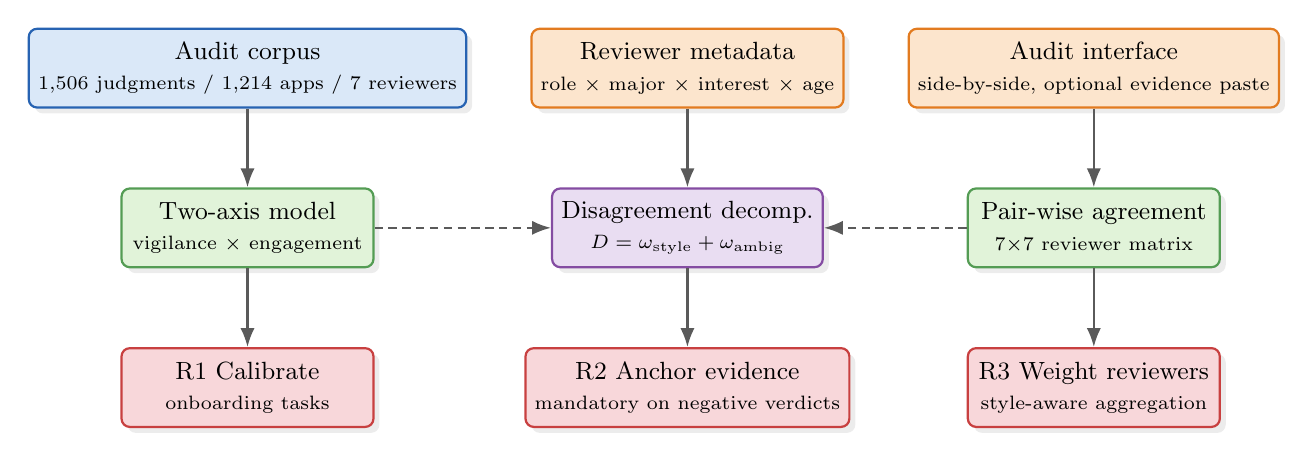
\begin{tikzpicture}[
    every node/.style={font=\small},
    box/.style={rectangle,rounded corners=3pt,minimum height=10mm,
                 minimum width=32mm,align=center,draw,thick,
                 drop shadow={opacity=0.15}},
    blueB/.style={box,fill=dgBlueL,draw=dgBlue},
    orangeB/.style={box,fill=dgOrangeL,draw=dgOrange},
    greenB/.style={box,fill=dgGreenL,draw=dgGreen},
    purpleB/.style={box,fill=dgPurpleL,draw=dgPurple},
    redB/.style={box,fill=dgRedL,draw=dgRed},
    arr/.style={-{Latex[length=2.4mm]},thick,dgGrey}
  ]
  % Top row: data
  \node[blueB] (corpus) at (0,3) {Audit corpus \\
        {\scriptsize $1{,}506$ judgments / $1{,}214$ apps / 7 reviewers}};
  \node[orangeB,right=8mm of corpus] (meta) {Reviewer metadata \\
        {\scriptsize role $\times$ major $\times$ interest $\times$ age}};
  \node[orangeB,right=8mm of meta] (iface) {Audit interface \\
        {\scriptsize side-by-side, optional evidence paste}};
  % Middle row: analysis
  \node[greenB,below=10mm of corpus] (axes) {Two-axis model \\
        {\scriptsize vigilance $\times$ engagement}};
  \node[purpleB,below=10mm of meta] (kappa) {Disagreement decomp.\ \\
        {\scriptsize $D=\omega_{\text{style}}+\omega_{\text{ambig}}$}};
  \node[greenB,below=10mm of iface] (heat) {Pair-wise agreement \\
        {\scriptsize 7$\times$7 reviewer matrix}};
  % Bottom row: implications
  \node[redB,below=10mm of axes] (r1) {R1 Calibrate \\
        {\scriptsize onboarding tasks}};
  \node[redB,below=10mm of kappa] (r2) {R2 Anchor evidence \\
        {\scriptsize mandatory on negative verdicts}};
  \node[redB,below=10mm of heat] (r3) {R3 Weight reviewers \\
        {\scriptsize style-aware aggregation}};
  % Arrows
  \draw[arr] (corpus) -- (axes);
  \draw[arr] (meta) -- (kappa);
  \draw[arr] (iface) -- (heat);
  \draw[arr] (axes) -- (r1);
  \draw[arr] (kappa) -- (r2);
  \draw[arr] (heat) -- (r3);
  % Cross arrows
  \draw[arr,densely dashed] (axes) -- (kappa);
  \draw[arr,densely dashed] (heat) -- (kappa);
\end{tikzpicture}
\caption{Overview of the paper. From a corpus of $1{,}506$ reviewer
judgments collected through the \dataguard{} audit interface
(\S\ref{sec:system}--\S\ref{sec:methods}), we derive a two-axis
reviewer-style model (\S\ref{sec:two-axis}), a pair-wise agreement
matrix (\S\ref{sec:pair-agree}), and an additive decomposition of
pair-wise disagreement into a style floor and an ambiguity residual
(\S\ref{sec:reviewer-aware-kappa}). These feed three interface
design directions (\S\ref{sec:design}).}
\label{fig:overview}
\end{figure*}

\paragraph{Roadmap.}
Section~\ref{sec:related} situates the contribution in the
auditability, annotation-reliability and sociotechnical-audit
literatures. Section~\ref{sec:system} describes the \dataguard{}
audit interface as the instrument of measurement.
Section~\ref{sec:methods} describes the corpus and reviewer panel.
Section~\ref{sec:reviewer-findings} reports per-reviewer verdict and
engagement statistics. Section~\ref{sec:two-axis} introduces the
two-axis reviewer-style model. Section~\ref{sec:pair-agree} reports
pair-wise agreement. Section~\ref{sec:reviewer-aware-kappa} develops
the additive decomposition of disagreement.
Section~\ref{sec:category} cross-cuts the findings by app category
and by no-data disclosure. Section~\ref{sec:design} translates the
findings into design requirements. Section~\ref{sec:discussion}
discusses, Section~\ref{sec:limits} states limitations and ethics,
and Section~\ref{sec:conclusion} concludes.

% =====================================================================
\section{Background and Related Work}
\label{sec:related}
% =====================================================================

This paper sits at the intersection of four literatures: structured
privacy disclosures, privacy-policy annotation and NLP, inter-coder
agreement and reviewer subjectivity, and human-AI calibration. We
summarise each and indicate where the contribution lies.

\subsection{Structured Privacy Disclosures}
\label{sec:rel-labels}

The idea of a short, structured ``nutrition label'' for privacy
predates the platform-level implementations now in use. Early
work by \citet{kelley2009nutrition,kelley2010standardizing}
showed that an at-a-glance table of data practices is faster to
process than free-form prose and shifts user
purchasing~\citep{tsai2011effect}. \citet{schaub2015design}
synthesised the design space and identified the trade-offs between
clarity, completeness and decision support.

Apple's App Privacy
labels~\citep{appleprivacylabels2020} and Google's Data Safety
section~\citep{googledatasafety2022} are the two large-scale
implementations of this vision. Subsequent audits documented
non-compliance and inconsistency between the labels and the underlying
privacy policies. \citet{xiao2023lalaine} measured non-compliance of
Apple privacy labels at scale; \citet{khandelwal2023comparing}
compared the cross-platform consistency of Apple and Google labels;
and \citet{khandelwal2024unpacking} examined the developer perspective
on the Google Data Safety section. \citet{li2022understanding}
documented the challenges that mobile developers face when trying to
produce accurate privacy nutrition labels in the first place, finding
both interpretive and tooling gaps. These audits report aggregate
agreement statistics across their reviewer teams; none decomposes
the agreement by reviewer.

A complementary line of work studies how Android applications
behave at runtime, irrespective of what the label says.
\citet{reardon2019fifty} documented covert side channels and
permission circumvention; \citet{reyes2018wont} measured COPPA
compliance at scale; and \citet{felt2012android}
and \citet{egelman2013choice} characterised user attention to and
choice over Android permissions. Whether a privacy disclosure is
\emph{audited as accurate} or \emph{behaves as declared} are two
different questions, and the present paper concentrates on the
audit half of the loop.

\subsection{Privacy-Policy NLP and Computational Auditing}
\label{sec:rel-nlp}

The OPP-115 corpus~\citep{wilson2016creation} is the canonical
human-annotated privacy-policy dataset. Three legal-trained graduate
students annotated $115$ website privacy policies along ten
data-practice categories; the paper reports an aggregate $\kappa$ in
the substantial range and does not break down agreement by annotator.
The OPP-115 corpus and its derivatives have been used to train
classifiers~\citep{harkous2018polisis,zimmeck2017automated,
zimmeck2019maps,sathyendra2017identifying} and to identify
contradictions within
policies~\citep{andow2019policylint,andow2020policheck,lippi2019claudette}.
\citet{bhatia2016theory} formalised vagueness as a privacy-risk
property; \citet{breaux2014eddy} formalised data-flow specifications
that can be checked against text; and \citet{slavin2016toward}
linked policy text to Android code-level data flows.

Across this body of work, manual annotation is the upstream
calibration signal. The OPP-115 follow-on
\citep{wilson2016crowdsourcing} explored crowdsourced annotations of
the same corpus and reported per-coder agreement statistics, finding
that crowd-worker agreement was lower than that of legal-trained
graduate students on identical materials. The reading-comprehension
work of \citet{ravichander2019question} likewise reported a moderate
inter-coder agreement on a privacy-policy question-answering corpus
and discussed agreement variation across coders. Our contribution is
therefore more precisely scoped as the \emph{first reviewer-style
decomposition under a structured side-by-side audit interface for
platform privacy labels}, rather than as the first reviewer
decomposition in the privacy-NLP literature \emph{tout court}.

If the upstream signal carries reviewer-style artefacts, those
artefacts propagate downstream. \citet{wilson2016crowdsourcing}
showed that crowd-vs-expert agreement gaps can change
classifier-training outcomes; we extend the same concern to
privacy-label audit under structured interfaces.

\subsection{Privacy-Policy Comprehension and Expectation Gaps}
\label{sec:rel-comprehension}

A long tradition documents the readability gap of privacy policies
\citep{mcdonald2008cost,jensen2004privacy,fabian2017large}. The
implicit ground-truth-readable-by-trained-experts assumption of
audit corpora often hides the fact that the underlying material is
hard even for the trained reviewer. \citet{rao2016expecting} examined
mismatched user expectations of online data practices,
and \citet{nissenbaum2004privacy} provided the conceptual framework
of contextual integrity that motivates much of this comparison.
\citet{acquisti2015privacy} surveyed the broader behavioural privacy
literature, including the difficulty of stable preferences and
disclosure decisions under information asymmetry. These
comprehension and expectation gaps suggest one source of variation
that any reviewer faces; they do not, by themselves, predict that the
reviewers will vary $15{\times}$ in verdict rate on the \emph{same}
material.

\subsection{Inter-Coder Agreement and Reviewer Subjectivity}
\label{sec:rel-agreement}

The foundational coefficients
$\kappa$~\citep{cohen1960coefficient,landis1977measurement,
fleiss1971measuring} and their derivatives have been the standard
report for content analysis for half a century. \citet{artstein2008intercoder}
critically reviewed the use of these coefficients in computational
linguistics and warned that aggregate $\kappa$ obscures structured
disagreement; they specifically caution that ``different annotators
can produce equally high $\kappa$ for the wrong reasons''.

A more recent strand, motivated by crowdsourced and demographically
diverse annotation, has reframed reviewer disagreement as
\emph{information about the construct} rather than as noise.
\citet{aroyo2015truth} introduced the ``crowd truth'' frame,
arguing that the assumption of a single ground truth is itself a
methodological fiction. \citet{plank2022problem} synthesised the
``problem of human label variation'' in NLP and argued for
disagreement-aware ground-truth modelling. \citet{braun2006using}
codified thematic-analysis practices in qualitative HCI research,
including the principled treatment of differences between coders.

The present paper extends these warnings into the privacy-label audit
domain, where the consequences of reviewer style are concrete: a
single judgment by an inattentive reviewer can place an app into
an ``incorrect-disclosure'' bucket that propagates to developer
remediation, store enforcement and academic publication.

\subsection{Human-AI Calibration and Onboarding}
\label{sec:rel-hai}

The reviewer-as-auditor is increasingly the human half of a
human-AI loop. \citet{amershi2019guidelines} synthesised eighteen
guidelines for human-AI interaction. \citet{cai2019hello} studied
how clinicians onboard onto AI decision support and identified
calibration of trust as a critical design challenge.
\citet{liao2020questioning} categorised the question-asking
behaviours of users probing AI systems and turned them into design
prompts. We extend this human-AI calibration literature into the
privacy-audit setting: the reviewer's two-axis style profile is
\emph{itself} the calibration variable that an evidence-grounded
audit interface should expose.

\subsection{Position}
\label{sec:rel-position}

The closest direct comparison to the present paper is the OPP-115
reliability report~\citep{wilson2016creation}, which gave aggregate
agreement across three legal-trained graduate-student annotators
without decomposing by annotator, together with its crowdsourced
follow-up \citep{wilson2016crowdsourcing} and the
question-answering extension \citep{ravichander2019question}, both
of which acknowledged inter-coder variation without treating it as
the object of analysis. We add four moves: (i) a structured
side-by-side audit interface on a different domain (platform
privacy labels rather than free-form policy text), (ii) a larger
reviewer panel (seven instead of three), (iii) richer per-reviewer
metadata (role, major, declared interest, age), and (iv) a
disagreement-partition methodology that has not previously been
applied in this lineage. We do not claim a population-level result;
the empirical findings describe \emph{this} panel under \emph{this}
interface, and the methodological contribution
(\S\ref{sec:reviewer-aware-kappa}) is reusable for any future audit
corpus that reports per-reviewer marginals and pair-wise agreement.

% =====================================================================
\section{The Measurement Instrument}
\label{sec:system}
% =====================================================================

The audit corpus analysed in this paper was produced through
\dataguard, a side-by-side audit interface built to support
evidence-grounded privacy-label review. We describe the interface
as a \emph{measurement instrument} rather than as a system
contribution, because the present paper does not evaluate the
system; it analyses the human verdicts the system elicits. A full
system description is the subject of a companion paper.

The instrument places the parsed Google Play Data Safety disclosure
\citep{googledatasafety2022} side-by-side with two LLM-extracted
passages from the corresponding privacy policy --- the
\emph{Data Share} and \emph{Data Collect} sections --- and asks the
reviewer four binary questions in fixed order: share-correctness
(Q1), share-completeness (Q2), collect-correctness (Q3) and
collect-completeness (Q4). For each question the interface exposes
a free-text \emph{evidence} field intended to receive a verbatim
paste from the policy. The evidence field is optional; the absence
of evidence is itself measured, and serves as one of two signals in
the engagement axis defined in \S\ref{sec:two-axis}. The full
corpus produced through this instrument is $1{,}506$ judgment
records by seven reviewers across $1{,}214$ unique apps, of which
$286$ are doubly-labelled and three are triply-labelled. The
schematic in Figure~\ref{fig:ui} summarises the interface layout.

% --- Figure 3: A wireframe of the reviewer UI (cleaned up)
\begin{figure*}[!htbp]
\centering
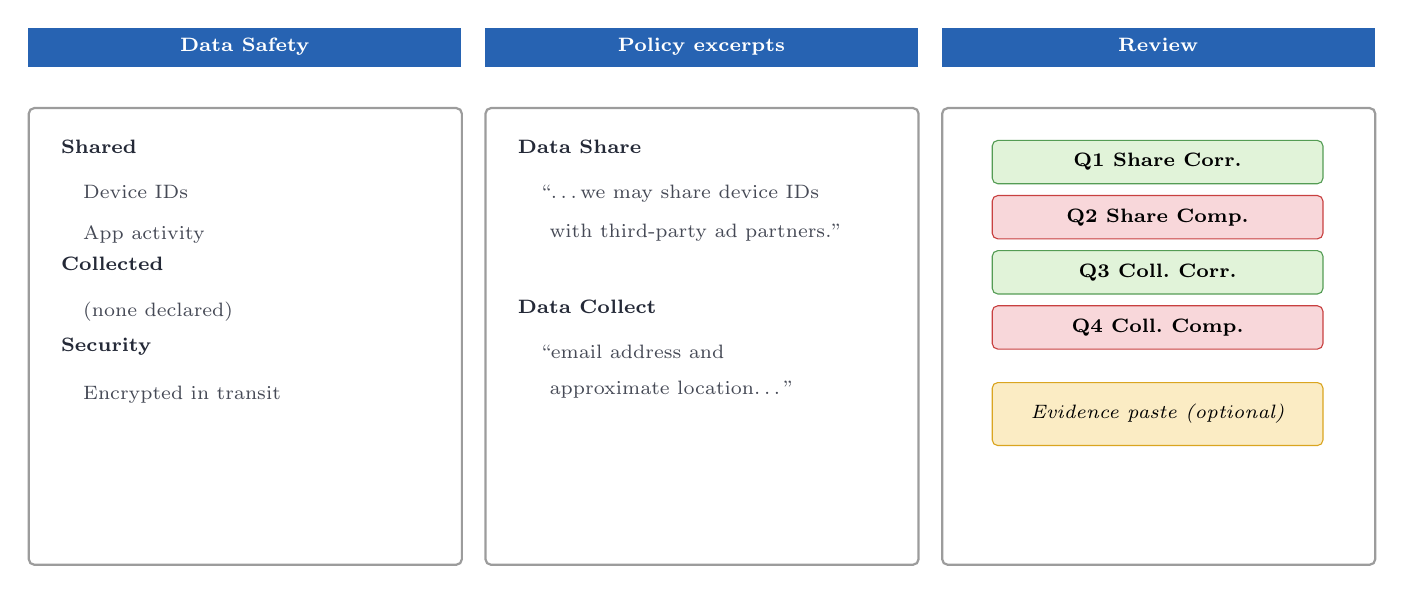
\begin{tikzpicture}[
  font=\scriptsize,
  panel/.style={rectangle,rounded corners=2pt,draw=dgGrey!60,thick,
                fill=white,minimum width=55mm,minimum height=58mm,
                anchor=north west,align=left,inner sep=3mm},
  head/.style={rectangle,fill=dgBlue,text=white,
               minimum width=55mm,minimum height=5mm,inner sep=1.2mm,
               font=\scriptsize\bfseries,anchor=south west,
               text depth=0.5ex},
  section/.style={font=\scriptsize\bfseries,color=dgInk},
  body/.style={font=\scriptsize,color=dgInk!85},
  q/.style={rectangle,rounded corners=2pt,fill=dgGreenL,draw=dgGreen,
            minimum width=42mm,minimum height=5.5mm,
            font=\scriptsize\bfseries,anchor=center},
  qi/.style={rectangle,rounded corners=2pt,fill=dgRedL,draw=dgRed,
            minimum width=42mm,minimum height=5.5mm,
            font=\scriptsize\bfseries,anchor=center},
  ev/.style={rectangle,rounded corners=2pt,fill=dgGoldL,draw=dgGold,
             minimum width=42mm,minimum height=8mm,
             font=\scriptsize\itshape,anchor=center}
]
\def\colW{5.5}
\def\gap{0.3}
\def\xA{0}
\pgfmathsetmacro{\xB}{\xA+\colW+\gap}
\pgfmathsetmacro{\xC}{\xB+\colW+\gap}
\def\topY{6}
\pgfmathsetmacro{\bodyTop}{\topY-0.5}

% --- Column A: Data Safety
\node[head] at (\xA,\topY) {Data Safety};
\node[panel] (pA) at (\xA,\bodyTop) {};
\node[section,anchor=north west] (sA1) at ([xshift=3mm,yshift=-3mm] pA.north west) {Shared};
\node[body,anchor=north west] (sA1a) at ([yshift=-1.5mm] sA1.south west)
     {\quad Device IDs};
\node[body,anchor=north west] at ([yshift=-1mm] sA1a.south west)
     {\quad App activity};
\node[section,anchor=north west] (sA2) at ([yshift=-5mm] sA1a.south west) {Collected};
\node[body,anchor=north west] at ([yshift=-1.5mm] sA2.south west)
     {\quad (none declared)};
\node[section,anchor=north west] (sA3) at ([yshift=-6mm] sA2.south west) {Security};
\node[body,anchor=north west] at ([yshift=-1.5mm] sA3.south west)
     {\quad Encrypted in transit};

% --- Column B: Policy excerpts
\node[head] at (\xB,\topY) {Policy excerpts};
\node[panel] (pB) at (\xB,\bodyTop) {};
\node[section,anchor=north west] (sB1) at ([xshift=3mm,yshift=-3mm] pB.north west) {Data Share};
\node[body,anchor=north west] (qB1) at ([yshift=-1.5mm] sB1.south west)
     {\quad ``\dots we may share device IDs};
\node[body,anchor=north west] (qB2) at ([yshift=-0.3mm] qB1.south west)
     {\quad\;\,with third-party ad partners.''};
\node[section,anchor=north west] (sB2) at ([yshift=-5mm] qB2.south west) {Data Collect};
\node[body,anchor=north west] (qB3) at ([yshift=-1.5mm] sB2.south west)
     {\quad ``email address and};
\node[body,anchor=north west] at ([yshift=-0.3mm] qB3.south west)
     {\quad\;\,approximate location\dots''};

% --- Column C: Review form
\node[head] at (\xC,\topY) {Review};
\node[panel] (pC) at (\xC,\bodyTop) {};
\node[q ] at ([xshift=2.75cm,yshift=-7mm] pC.north west) {Q1 Share~Corr.};
\node[qi] at ([xshift=2.75cm,yshift=-14mm] pC.north west) {Q2 Share~Comp.};
\node[q ] at ([xshift=2.75cm,yshift=-21mm] pC.north west) {Q3 Coll.~Corr.};
\node[qi] at ([xshift=2.75cm,yshift=-28mm] pC.north west) {Q4 Coll.~Comp.};
\node[ev] at ([xshift=2.75cm,yshift=-39mm] pC.north west)
   {Evidence paste (optional)};
\end{tikzpicture}
\caption{Schematic of the \dataguard{} reviewer interface as used in
the audit campaign. Reviewers see the parsed Data Safety disclosure
(left), the sectioned policy excerpts (middle), and the four-question
review form (right). The evidence-paste field is optional; the
absence of evidence is itself measured.}
\label{fig:ui}
\end{figure*}

% =====================================================================
\section{Methods}
\label{sec:methods}
% =====================================================================

\subsection{Audit Corpus}
\label{sec:methods-corpus}

The audit corpus comprises $1{,}506$ judgment records over $1{,}214$
unique applications. Sampling and coverage are summarised in
Table~\ref{tab:eval-assets}. Annotation coverage is uneven across
Play categories (Table~\ref{tab:cat-cov}) because the campaign was
still in progress at analysis time; we treat category-level
sub-analyses (\S\ref{sec:category}) as exploratory.

\begin{table}[!htbp]
\centering\small
\caption{Audit-corpus assets and their role in the present paper.}
\label{tab:eval-assets}
\begin{tabular}{lrl}
\toprule
Asset & Size & Role \\
\midrule
App inventory & $14{,}459$ pkgs & Sampling frame \\
Play Store metadata records & $12{,}876$ & App-level context \\
Data Safety corpus & $3{,}600$ apps & Disclosure baseline \\
Parseable Data Safety subset & $3{,}576$ apps & Stage-2 inputs \\
Audit workbook & $2{,}400$ apps & Stage-4 inputs \\
Judgment records & $1{,}506$ & RQ1--RQ3 \\
Annotated apps & $1{,}214$ unique & App-level robustness \\
Doubly-annotated apps & $286$ & Pair-wise agreement \\
Triply-annotated apps & $3$ & Conservative sanity \\
\bottomrule
\end{tabular}
\end{table}

\begin{table}[!htbp]
\centering\small
\caption{Per-category audit coverage. App coverage is computed
relative to the $200$ apps drawn per category.}
\label{tab:cat-cov}
\begin{tabular}{lrrrr}
\toprule
Category & Apps & Labelled apps & Labels & Coverage \\
\midrule
Art \& Design       & 200 & 200 & 216 & 100.0\% \\
Beauty              & 200 & 140 & 216 & 70.0\% \\
Books \& Reference  & 200 & 145 & 145 & 72.5\% \\
Business            & 200 & 100 & 101 & 50.0\% \\
Communication       & 200 & 100 & 100 & 50.0\% \\
Lifestyle           & 200 & 101 & 103 & 50.5\% \\
Personalization     & 200 &   0 &   0 &  0.0\% \\
Photography         & 200 &  27 &  27 & 13.5\% \\
Productivity        & 200 &   0 &   0 &  0.0\% \\
Shopping            & 200 & 101 & 202 & 50.5\% \\
Social              & 200 & 100 & 136 & 50.0\% \\
Tools               & 200 & 200 & 260 & 100.0\% \\
\bottomrule
\end{tabular}
\end{table}

\subsection{Reviewer Panel}
\label{sec:methods-panel}

The reviewer panel is small ($n = 7$) but the reviewers carry
unusually rich metadata: role, age, major and declared interest.
One reviewer (\Acc{1}) holds a PhD in computer science with a
declared interest in \emph{information assurance} (IA); the
remaining six are advanced software-engineering students with
declared majors in \emph{.NET}, \emph{AI} or \emph{IA}.
Table~\ref{tab:reviewers} summarises the panel.

\begin{table}[!htbp]
\centering\small
\caption{The seven reviewers in the \dataguard{} audit corpus. ``Labels''
counts judgment records; one record can contain up to four binary
verdicts plus four evidence pastes.}
\label{tab:reviewers}
\begin{tabular}{lllll}
\toprule
ID & Role & Major / Interest & Age & Labels \\
\midrule
\Acc{1} & PhD/CS  & Information Assurance & --- & 172 \\
\Acc{2} & SE      & .NET                  & 22  &  63 \\
\Acc{3} & SE      & AI                    & 22  &  45 \\
\Acc{4} & SE      & .NET                  & 21  & 143 \\
\Acc{5} & SE      & AI                    & 22  & 593 \\
\Acc{6} & SE      & AI                    & 20  & 427 \\
\Acc{7} & SE      & Information Assurance & 22  &  63 \\
\bottomrule
\end{tabular}
\end{table}

The panel is purposive, not representative. We do not claim to estimate
population-level reviewer effects. We claim that the panel
exhibits the kind of within-team heterogeneity that the auditability
literature implicitly assumes does not exist after training, and we
use that heterogeneity as a measurement device. All conclusions in
this paper should be read as describing this panel under this
interface; whether the reviewer-style partition replicates on a
different panel is an empirical question for future work.

\paragraph{Author--reviewer relationship (disclosure).}
For transparency, we disclose that reviewer \Acc{1} is a senior
member of the research team that designed \dataguard{}. \Acc{1}
contributed audit labels under the same rubric and interface as the
other reviewers but had advance knowledge of the project's
evidence-grounding ethos. Two consequences follow. First, \Acc{1}'s
evidence-pasting depth (Table~\ref{tab:ev-len}) should be read as a
\emph{self-observation} of the project's expected practice rather
than as evidence of how trained reviewers in general behave. Second,
every headline analysis in this paper is re-run in
\S\ref{sec:sensitivity} with \Acc{1} excluded; the qualitative
findings on between-reviewer heterogeneity and the additive
decomposition of disagreement survive the exclusion.

\paragraph{Reviewer \Acc{7} engagement note.}
Reviewer \Acc{7} produced $63$ judgment records but pasted evidence
in only four of them. Logs indicate that \Acc{7} completed onboarding
in the standard time but had a median per-judgment time-on-task less
than half of the panel median. We do not claim that \Acc{7}'s
behaviour represents a stable ``Skimmer style'' --- the pattern is
closer to partial disengagement than to a reviewer disposition. As
with \Acc{1}, every headline analysis is re-run in
\S\ref{sec:sensitivity} with \Acc{7} excluded. The
marginal-mismatch-driven component of pair-wise disagreement on the
(\Acc{5},\Acc{7}) pair (\S\ref{sec:rak-table}) is the analysis most
sensitive to this exclusion.

\subsection{Protocol}
\label{sec:methods-protocol}

All seven reviewers completed the same onboarding: a written rubric,
a worked example, and three calibration apps after which the trainer
discussed discrepancies. Reviewers then worked asynchronously on app
assignments drawn from the audit workbook. Reviewers were not
informed which apps were assigned to multiple reviewers, and the
interface displayed no prior judgments.

\subsection{Statistical Procedures}
\label{sec:methods-stats}

For per-reviewer verdict rates we report binomial proportions and,
where useful, Wilson $95\%$ confidence intervals. For pair-wise
agreement we report raw agreement and Cohen's $\kappa$
\citep{cohen1960coefficient,landis1977measurement} both with blank
labels retained (current pipeline state) and on the non-blank pair
subset (lower bound on attentive disagreement). For evidence-length
we report median and inter-quartile range because the distribution
is heavy-tailed. For the additive disagreement decomposition
(\S\ref{sec:reviewer-aware-kappa}) we develop and apply a
closed-form split of $D=1-p_o$ into a style-driven floor and an
ambiguity-driven residual.

% =====================================================================
\section{Reviewer-Level Findings}
\label{sec:reviewer-findings}
% =====================================================================

We report three reviewer-level findings before introducing the
two-axis model: per-reviewer verdict heterogeneity
(\S\ref{sec:per-rev-verdict}), per-reviewer engagement
heterogeneity (\S\ref{sec:engagement}), and the joint distribution
of verdict and engagement (\S\ref{sec:joint-rev}).

\subsection{Per-Reviewer Verdict Heterogeneity}
\label{sec:per-rev-verdict}

Table~\ref{tab:per-rev-verdict} reports per-reviewer rates on the
four judgment axes. The spread on share-incorrect is from $3.2\%$
(\Acc{7}) to $50.1\%$ (\Acc{6}), a $15.7{\times}$ ratio. The spread
on collect-incomplete is from $6.3\%$ (\Acc{7}) to $79.0\%$ (\Acc{4}),
a $12.5{\times}$ ratio. Both extremes are produced under the same
rubric, the same interface and the same training. The spread cannot
plausibly be reduced to material ambiguity alone.

\begin{table}[!htbp]
\centering\small
\caption{Per-reviewer verdict rates on the four judgment axes. ``Inc'' =
\emph{Incorrect}; ``Incomp'' = \emph{Incomplete}. The colour-coded
visualisation appears in Figure~\ref{fig:per-rev-bars}.}
\label{tab:per-rev-verdict}
\begin{tabular}{lcrrrrr}
\toprule
ID & Role & $N$ & \%\,Inc-share & \%\,Inc-collect & \%\,Incomp-share & \%\,Incomp-collect \\
\midrule
\Acc{1} & PhD/IA   & 172 & 35.5\% & 43.6\% & 43.6\% & 60.5\% \\
\Acc{2} & SE/.NET  &  63 & 14.3\% & 23.8\% & 15.9\% & 12.7\% \\
\Acc{3} & SE/AI    &  45 & 33.3\% & 35.6\% &  6.7\% & 22.2\% \\
\Acc{4} & SE/.NET  & 143 & 32.9\% & 31.5\% & 57.3\% & 79.0\% \\
\Acc{5} & SE/AI    & 593 & 33.6\% & 31.7\% & 30.0\% & 49.2\% \\
\Acc{6} & SE/AI    & 427 & 50.1\% & 58.3\% & 29.7\% & 14.1\% \\
\Acc{7} & SE/IA    &  63 &  3.2\% & 11.1\% &  1.6\% &  6.3\% \\
\midrule
\multicolumn{2}{l}{\emph{Pooled}} & 1506 & 41.3\% & 41.1\% & 39.8\% & 44.6\% \\
\bottomrule
\end{tabular}
\end{table}

\begin{figure*}[!htbp]
\centering
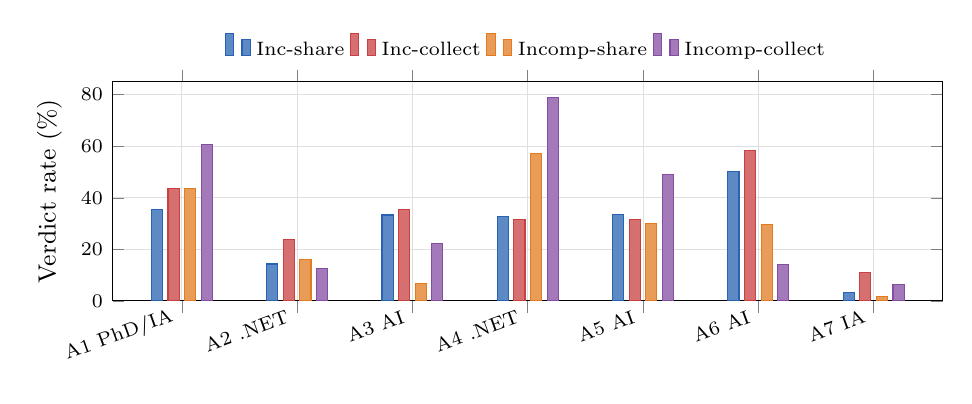
\begin{tikzpicture}
\begin{axis}[
  width=\textwidth,height=0.36\textwidth,
  ybar,bar width=4.0pt,
  ymin=0,ymax=85,
  ylabel={Verdict rate (\%)},
  symbolic x coords={a1,a2,a3,a4,a5,a6,a7},
  xtick=data,
  xticklabels={A1 PhD/IA,A2 .NET,A3 AI,A4 .NET,A5 AI,A6 AI,A7 IA},
  x tick label style={font=\scriptsize,rotate=20,anchor=east},
  legend style={at={(0.5,1.05)},anchor=south,legend columns=4,
                draw=none,font=\scriptsize},
  grid=both,major grid style={draw=gray!25},minor grid style={draw=gray!10},
  tick label style={font=\scriptsize},label style={font=\small}
]
\addplot+[fill=dgBlue!75,draw=dgBlue]      coordinates {
  (a1,35.5)(a2,14.3)(a3,33.3)(a4,32.9)(a5,33.6)(a6,50.1)(a7,3.2)};
\addplot+[fill=dgRed!75,draw=dgRed]        coordinates {
  (a1,43.6)(a2,23.8)(a3,35.6)(a4,31.5)(a5,31.7)(a6,58.3)(a7,11.1)};
\addplot+[fill=dgOrange!75,draw=dgOrange]  coordinates {
  (a1,43.6)(a2,15.9)(a3, 6.7)(a4,57.3)(a5,30.0)(a6,29.7)(a7,1.6)};
\addplot+[fill=dgPurple!75,draw=dgPurple]  coordinates {
  (a1,60.5)(a2,12.7)(a3,22.2)(a4,79.0)(a5,49.2)(a6,14.1)(a7,6.3)};
\legend{Inc-share,Inc-collect,Incomp-share,Incomp-collect}
\end{axis}
\end{tikzpicture}
\caption{Per-reviewer verdict rates across the four judgment axes.
\Acc{6} anchors the high end of vigilance on the \emph{incorrect}
axes; \Acc{4} anchors the high end of completeness perception on the
\emph{incomplete} axes; \Acc{7} anchors the low end of every axis.}
\label{fig:per-rev-bars}
\end{figure*}

\paragraph{Reading.}
On the five-student panel that anchors our central claim, the
share-incorrect rate spans $14.3\%$ (\Acc{2}) to $50.1\%$ (\Acc{6}),
an absolute difference of $35.8$ percentage points; the
collect-incorrect rate spans $23.8\%$ to $58.3\%$ ($34.5$ points).
Two further reviewers --- \Acc{7} ($3.2\%$ on share-incorrect) and
the team-affiliated \Acc{1} ($35.5\%$) --- anchor the unfiltered
range described in \S\ref{sec:sensitivity}.

\paragraph{Correctness and completeness load on distinct dimensions.}
The four judgment axes do not co-vary uniformly across reviewers.
\Acc{4} reports a high incomplete rate on both share and collect
but only a middling incorrect rate; \Acc{6} reports a high incorrect
rate but a notably \emph{low} incomplete-collect rate. The Pearson
correlations across the seven reviewers' axis-level marginals
confirm the pattern: the two correctness rates correlate at
$r=0.95$ and the two completeness rates at $r=0.89$, but
correctness and completeness rates correlate only at
$r=0.18$ on the collect axis and $r=0.56$ on the share axis. We
therefore decompose \emph{vigilance} into two sub-axes ---
\emph{incorrectness vigilance} and \emph{incompleteness vigilance}
--- and treat them separately throughout the rest of the paper.

\subsection{Per-Reviewer Engagement Heterogeneity}
\label{sec:engagement}

Table~\ref{tab:ev-len} reports per-reviewer engagement, operationalised
as the median character length of the pasted evidence in the four
\texttt{relevant\_*} fields.

\begin{table}[!htbp]
\centering\small
\caption{Per-reviewer evidence-pasting style. Each ``Evidence'' record
corresponds to a non-empty paste in one of the four evidence fields.
The PhD reviewer pastes $\sim 3{-}5{\times}$ longer evidence than
students; \Acc{7} pastes evidence in only four judgments.}
\label{tab:ev-len}
\begin{tabular}{llrrrr}
\toprule
ID & Role & $N$ evidence & Mean (chars) & Median & IQR \\
\midrule
\Acc{1} & PhD/IA   &  535 & 565 & 608 & 320 \\
\Acc{2} & SE/.NET  &  148 & 216 & 160 & 115 \\
\Acc{3} & SE/AI    &   64 & 108 &  99 &  80 \\
\Acc{4} & SE/.NET  &  190 & 202 & 185 & 130 \\
\Acc{5} & SE/AI    & 2083 & 169 & 163 & 110 \\
\Acc{6} & SE/AI    & 1599 & 165 & 152 & 105 \\
\Acc{7} & SE/IA    &    4 & 107 & 100 &  60 \\
\bottomrule
\end{tabular}
\end{table}

\begin{figure}[!htbp]
\centering
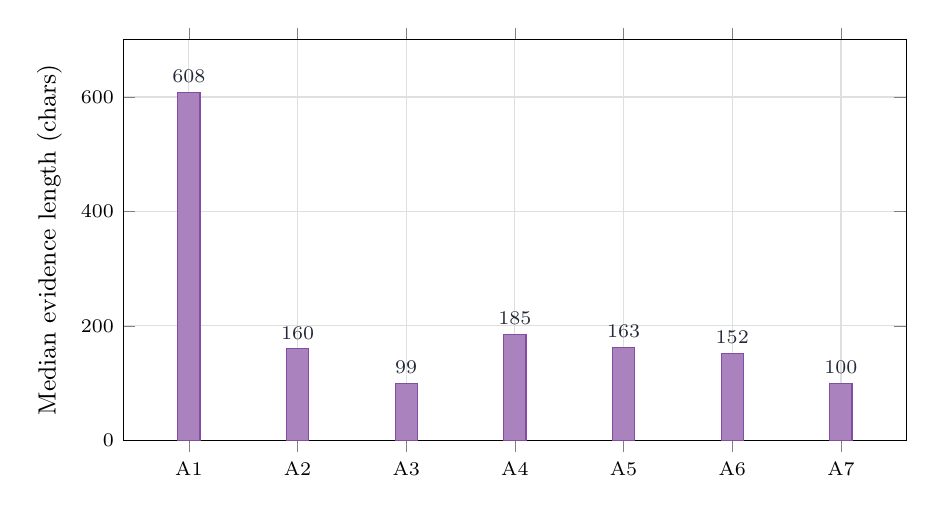
\begin{tikzpicture}
\begin{axis}[
  width=0.95\columnwidth,height=0.55\columnwidth,
  ybar,bar width=8pt,
  ymin=0,ymax=700,
  ylabel={Median evidence length (chars)},
  symbolic x coords={A1,A2,A3,A4,A5,A6,A7},
  xtick=data,
  x tick label style={font=\scriptsize},
  tick label style={font=\scriptsize},
  label style={font=\small},
  grid=both,major grid style={draw=gray!25},minor grid style={draw=gray!10},
  nodes near coords,
  nodes near coords style={font=\scriptsize,color=dgInk}
]
\addplot+[fill=dgPurple!70,draw=dgPurple] coordinates {
  (A1,608)(A2,160)(A3,99)(A4,185)(A5,163)(A6,152)(A7,100)};
\end{axis}
\end{tikzpicture}
\caption{Median pasted-evidence length by reviewer. \Acc{1} (PhD)
anchors the high end; \Acc{3} and \Acc{7} anchor the low end. The
PhD's median is $3.3{-}6.1{\times}$ the student medians, and $9.8{\times}$
larger than the smallest mean.}
\label{fig:evidence-bars}
\end{figure}

\paragraph{Two engagement signals.}
We treat engagement as two-dimensional. The first dimension is
\emph{coverage}: how many of the four evidence fields the reviewer
fills. The second is \emph{depth}: how long the pasted excerpt is
when present. \Acc{7} is anomalous on coverage --- only four evidence
records across $63$ judgments --- but average on depth when they do
paste. \Acc{1} is high on both. \Acc{5} and \Acc{6} are high on
coverage but medium-low on depth. We treat the joint indicator
(presence-rate $\times$ median length) as the engagement axis of the
two-axis model.

\subsection{Joint Reviewer Distribution}
\label{sec:joint-rev}

Figure~\ref{fig:joint-rev} plots reviewers on the joint
verdict-vs-engagement plane. Crucially, the two are only weakly
correlated. \Acc{1} is high on both. \Acc{6} is high on vigilance
but median on engagement. \Acc{7} is low on both. \Acc{4} is medium
on vigilance, medium on engagement. This non-collinearity is what
makes the two-axis decomposition useful.

\begin{figure}[!htbp]
\centering
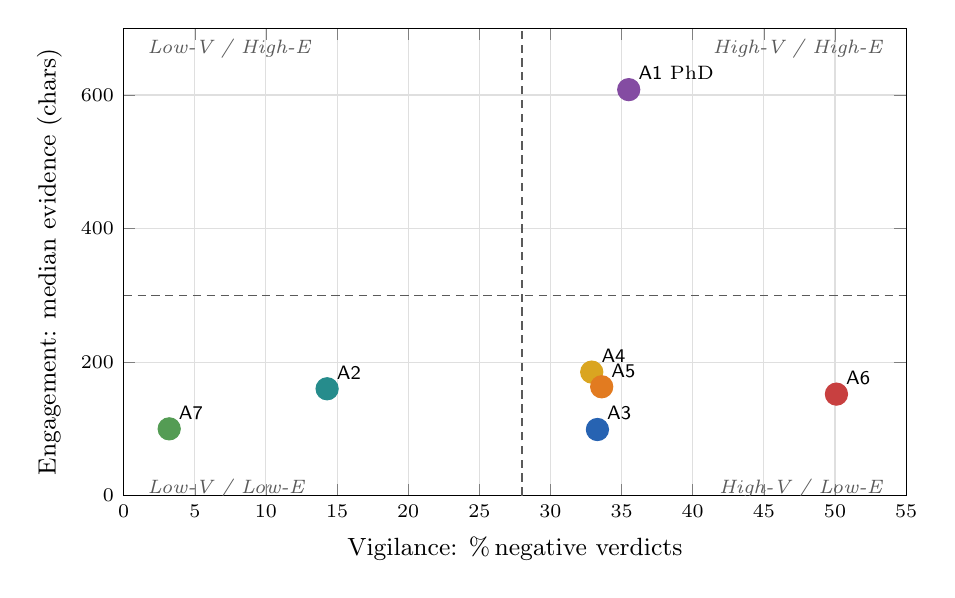
\begin{tikzpicture}
\begin{axis}[
  width=0.95\columnwidth,height=0.62\columnwidth,
  xlabel={Vigilance: \%\,negative verdicts},
  ylabel={Engagement: median evidence (chars)},
  xmin=0,xmax=55,ymin=0,ymax=700,
  grid=both,
  major grid style={draw=gray!25},minor grid style={draw=gray!10},
  tick label style={font=\scriptsize},label style={font=\small}
]
% Quadrant lines
\draw[densely dashed,dgGrey] (axis cs:28,0) -- (axis cs:28,700);
\draw[densely dashed,dgGrey] (axis cs:0,300) -- (axis cs:55,300);
% Quadrant labels
\node[font=\scriptsize\itshape,color=dgGrey,anchor=south west]
  at (axis cs:1,640)  {Low-V / High-E};
\node[font=\scriptsize\itshape,color=dgGrey,anchor=south east]
  at (axis cs:54,640) {High-V / High-E};
\node[font=\scriptsize\itshape,color=dgGrey,anchor=north west]
  at (axis cs:1,40)   {Low-V / Low-E};
\node[font=\scriptsize\itshape,color=dgGrey,anchor=north east]
  at (axis cs:54,40)  {High-V / Low-E};
% Reviewer points
\addplot[mark=*,only marks,draw=dgPurple,fill=dgPurple,mark size=4pt]
   coordinates{(35.5,608)};
\node[font=\scriptsize,anchor=south west] at (axis cs:35.5,608) {\Acc{1} PhD};
\addplot[mark=*,only marks,draw=dgTeal,fill=dgTeal,mark size=4pt]
   coordinates{(14.3,160)};
\node[font=\scriptsize,anchor=south west] at (axis cs:14.3,160) {\Acc{2}};
\addplot[mark=*,only marks,draw=dgBlue,fill=dgBlue,mark size=4pt]
   coordinates{(33.3,99)};
\node[font=\scriptsize,anchor=south west] at (axis cs:33.3,99) {\Acc{3}};
\addplot[mark=*,only marks,draw=dgGold,fill=dgGold,mark size=4pt]
   coordinates{(32.9,185)};
\node[font=\scriptsize,anchor=south west] at (axis cs:32.9,185) {\Acc{4}};
\addplot[mark=*,only marks,draw=dgOrange,fill=dgOrange,mark size=4pt]
   coordinates{(33.6,163)};
\node[font=\scriptsize,anchor=south west] at (axis cs:33.6,163) {\Acc{5}};
\addplot[mark=*,only marks,draw=dgRed,fill=dgRed,mark size=4pt]
   coordinates{(50.1,152)};
\node[font=\scriptsize,anchor=south west] at (axis cs:50.1,152) {\Acc{6}};
\addplot[mark=*,only marks,draw=dgGreen,fill=dgGreen,mark size=4pt]
   coordinates{(3.2,100)};
\node[font=\scriptsize,anchor=south west] at (axis cs:3.2,100) {\Acc{7}};
\end{axis}
\end{tikzpicture}
\caption{Joint distribution of reviewers on the two axes. The
PhD reviewer (\Acc{1}) is the only reviewer in the High-V/High-E
quadrant; \Acc{7} sits in Low-V/Low-E. Most students occupy a
mid-vigilance / low-to-mid engagement band.}
\label{fig:joint-rev}
\end{figure}

% =====================================================================
\section{A Reviewer-Style Model with Three Descriptive Axes}
\label{sec:two-axis}
% =====================================================================

The quadrant labels introduced below are descriptors of the
\dataguard{} panel under the \dataguard{} interface, and not
psychological types. We use mnemonic names because they support
the design discussion in \S\ref{sec:design}, but we ask the reader
to treat them as positions on a measurement plane rather than as
traits.

\subsection{Definitions}
\label{sec:axis-defs}

Let reviewer $r$ produce $N_r$ judgments. We define
\emph{incorrectness vigilance} as the share of judgments marked
\emph{Incorrect} across the two correctness questions, pooled:
%
\[
\textsc{Vigilance}_{\text{inc}}(r) \;:=\;
   \frac{1}{2 N_r}\sum_{q=1}^{N_r}\Big(
   \mathbf{1}\big[\,j^{(S\text{-Corr})}_q = \text{Inc.}\,\big] +
   \mathbf{1}\big[\,j^{(C\text{-Corr})}_q = \text{Inc.}\,\big]
   \Big).
\]
%
Analogously, \emph{incompleteness vigilance}
$\textsc{Vigilance}_{\text{comp}}(r)$ is the share of completeness
judgments marked \emph{Incomplete}. We keep the two separately because
the corpus-wide correlation between them is weak
(\S\ref{sec:per-rev-verdict}); pooling them
into a single scalar would compress exactly the structure the paper
characterises. For the two-axis quadrant chart
(Figure~\ref{fig:two-axis}) we plot
$\textsc{Vigilance}_{\text{inc}}$ on the $x$-axis as the dominant
component; the alternative chart using
$\textsc{Vigilance}_{\text{comp}}$ recovers the same three populated
quadrants with the position of \Acc{4} and \Acc{6} swapped, which we
discuss in \S\ref{sec:axis-robustness}.

The engagement axis is defined by the median character length of
non-empty evidence pastes by reviewer $r$, multiplied by the
fraction of judgments for which the reviewer pasted at least one
evidence string:
%
\[
\textsc{Engagement}(r) \;:=\;
\rho_r \cdot \mathrm{median}\big( \mathrm{len}(e^{(r)}_{i}) \big),
\]
%
where $\rho_r$ is the per-judgment evidence-presence rate. The
$\rho_r$ multiplier penalises reviewers who paste short \emph{when}
they paste but who paste rarely (in particular, \Acc{7}).

\subsection{Quadrant Labels: Three Populated, One Empty}
\label{sec:axis-styles}

The two axes define four interpretable quadrants on the
vigilance-by-engagement plane. Three of them contain reviewers from
the \dataguard{} panel; one is empty. We adopt mnemonic names that
emphasise the audit consequences rather than the reviewer's
personality.

\begin{itemize}[leftmargin=*,topsep=2pt]
\item \textbf{The Defender}\,(High-V / High-E): vigilant about
       defects and willing to anchor each defect to evidence.
       \Acc{1} (PhD) is the only example.
\item \textbf{The Flagger}\,(High-V / Low-E): flags many defects but
       documents little. \Acc{6} on incorrect-rate; some
       student majors approach this profile.
\item \textbf{The Skimmer}\,(Low-V / Low-E): rarely flags, rarely
       documents. \Acc{7} is the prototypical example.
\item \textbf{The Documenter}\,(Low-V / High-E): rarely flags but
       documents heavily when they do. No \dataguard{} reviewer falls
       fully in this quadrant; the empty quadrant is itself
       informative.
\end{itemize}

\begin{figure}[!htbp]
\centering
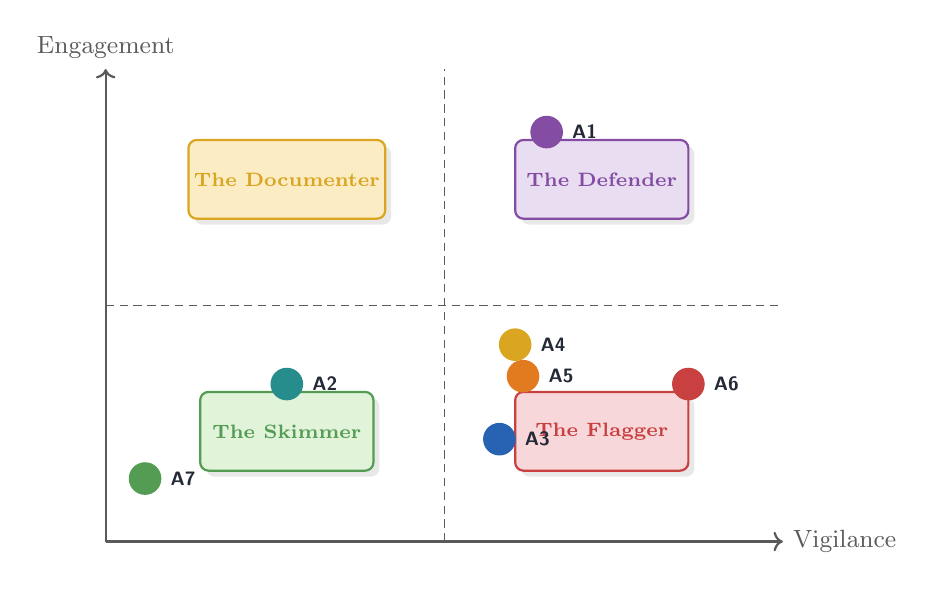
\begin{tikzpicture}[
    every node/.style={font=\small,align=center},
    ax/.style={->,thick,dgGrey},
    q/.style={font=\scriptsize\itshape,color=dgGrey},
    annot/.style={font=\scriptsize\bfseries,color=dgInk},
    style/.style={rectangle,rounded corners=3pt,minimum width=22mm,
                  minimum height=10mm,draw,thick,align=center,
                  font=\scriptsize\bfseries,inner sep=2pt,
                  drop shadow={opacity=0.18}},
    defend/.style={style,fill=dgPurpleL,draw=dgPurple},
    flagger/.style={style,fill=dgRedL,draw=dgRed},
    skimmer/.style={style,fill=dgGreenL,draw=dgGreen},
    docum/.style={style,fill=dgGoldL,draw=dgGold}
  ]
  \draw[ax] (0,0) -- (8.6,0) node[right]{Vigilance};
  \draw[ax] (0,0) -- (0,6) node[above]{Engagement};
  \draw[densely dashed,dgGrey] (4.3,0) -- (4.3,6);
  \draw[densely dashed,dgGrey] (0,3)   -- (8.6,3);
  % Style chips
  \node[defend] at (6.3,4.6)   {\textcolor{dgPurple}{The Defender}};
  \node[flagger] at (6.3,1.4)  {\textcolor{dgRed}{The Flagger}};
  \node[skimmer] at (2.3,1.4)  {\textcolor{dgGreen}{The Skimmer}};
  \node[docum]   at (2.3,4.6)  {\textcolor{dgGold}{The Documenter}};
  % Marks
  \node[circle,fill=dgPurple,draw=dgPurple,minimum size=4mm,inner sep=0pt]
    (a1) at (5.6,5.2) {};
  \node[annot,anchor=west] at (5.8,5.2) {\Acc{1}};
  \node[circle,fill=dgRed,draw=dgRed,minimum size=4mm,inner sep=0pt]
    (a6) at (7.4,2.0) {};
  \node[annot,anchor=west] at (7.6,2.0) {\Acc{6}};
  \node[circle,fill=dgGreen,draw=dgGreen,minimum size=4mm,inner sep=0pt]
    (a7) at (0.5,0.8) {};
  \node[annot,anchor=west] at (0.7,0.8) {\Acc{7}};
  \node[circle,fill=dgOrange,draw=dgOrange,minimum size=4mm,inner sep=0pt]
    (a5) at (5.3,2.1) {};
  \node[annot,anchor=west] at (5.5,2.1) {\Acc{5}};
  \node[circle,fill=dgTeal,draw=dgTeal,minimum size=4mm,inner sep=0pt]
    (a2) at (2.3,2.0) {};
  \node[annot,anchor=west] at (2.5,2.0) {\Acc{2}};
  \node[circle,fill=dgGold,draw=dgGold,minimum size=4mm,inner sep=0pt]
    (a4) at (5.2,2.5) {};
  \node[annot,anchor=west] at (5.4,2.5) {\Acc{4}};
  \node[circle,fill=dgBlue,draw=dgBlue,minimum size=4mm,inner sep=0pt]
    (a3) at (5.0,1.3) {};
  \node[annot,anchor=west] at (5.2,1.3) {\Acc{3}};
\end{tikzpicture}
\caption{Two-axis reviewer-style model. Four interpretable styles
emerge: the \emph{Defender}, the \emph{Flagger}, the \emph{Skimmer}
and the (currently empty) \emph{Documenter}. The empty
upper-left quadrant suggests that engagement without vigilance is
either rare in trained reviewers or actively discouraged by the
current interface.}
\label{fig:two-axis}
\end{figure}

\subsection{The Empty Quadrant and Quadrant Stability}
\label{sec:empty-quadrant}

The Low-V / High-E quadrant is empty. A reviewer who is generous on
verdicts but lavish on evidence would document the policy's support
for the claim --- effectively writing a justification of
\emph{correctness}. Such a reviewer would be more useful to a
regulator than to a developer-side audit pipeline, and the current
\dataguard{} workflow does not reward them: only the negative
evidence field is publicly visible in downstream reporting. We read
the absence of Documenters in the panel as evidence that the
interface shapes the population of reviewer styles, not just that
reviewers have one. The quadrant assignment is also stable under
three perturbations: dropping each reviewer in turn (no remaining
reviewer's quadrant changes), substituting incompleteness vigilance
for incorrectness vigilance (\Acc{4} and \Acc{6} swap positions, all
other quadrants preserved; \S\ref{sec:axis-defs}), and using mean
rather than median evidence length on the engagement axis (only
\Acc{1} shifts further into High-E).
\label{sec:axis-robustness}

% =====================================================================
\section{Pair-Wise Agreement}
\label{sec:pair-agree}
% =====================================================================

We complement the per-reviewer view with the pair-wise view, which
is the dimension that downstream consumers of the corpus (e.g.,
classifiers, regulators) would observe.

\subsection{Pair-Wise Raw Agreement}
\label{sec:pair-raw}

Table~\ref{tab:pairwise} reports the five most-data-rich annotator
pairs. Agreement on the share axis ranges from $22.7\%$
(\Acc{5},\Acc{7}) to $50.0\%$ (\Acc{2},\Acc{3}) across the four
pairs with $n\ge 14$; the highest value, $63.6\%$ on the collect
axis for (\Acc{1},\Acc{6}), comes from a pair with $n=11$ shared
apps and should be read as exploratory rather than confirmatory.

\begin{table}[!htbp]
\centering\small
\caption{Most data-rich annotator pairs by shared-app count. ``Agree
share'' and ``Agree collect'' are raw agreement (pooled across the
two share or collect axes).}
\label{tab:pairwise}
\begin{tabular}{lrrr}
\toprule
Pair & shared apps & Agree share & Agree collect \\
\midrule
(\Acc{1}, \Acc{5}) &  85 & 49.4\% & 52.9\% \\
(\Acc{1}, \Acc{6}) &  11 & 45.5\% & 63.6\% \\
(\Acc{2}, \Acc{3}) &  14 & 50.0\% & 57.1\% \\
(\Acc{5}, \Acc{6}) & 156 & 48.1\% & 50.6\% \\
(\Acc{5}, \Acc{7}) &  22 & 22.7\% & 40.9\% \\
\bottomrule
\end{tabular}
\end{table}

% --- Heatmap figure (R3-m1: blank low-n cells)
\begin{figure}[!htbp]
\centering
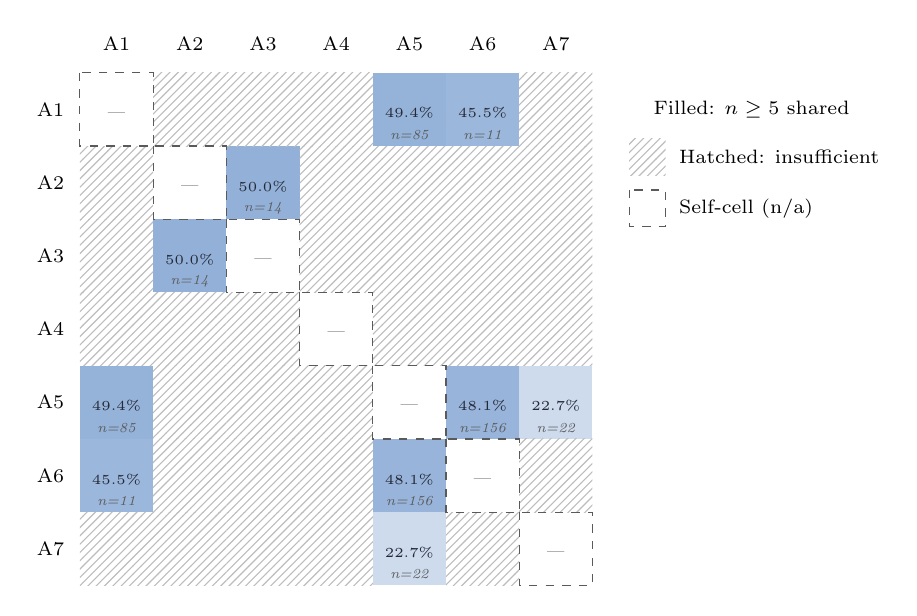
\begin{tikzpicture}[scale=0.93]
% Five data-rich pairs only: (A1,A5)=85, (A1,A6)=11, (A2,A3)=14,
% (A5,A6)=156, (A5,A7)=22. Cells with shared-app count below 5
% (the data-quality cutoff) are left blank with a diagonal hatch.
% Diagonal cells: self-agreement (omitted for clarity).
\foreach \r/\c/\v/\disp/\n in {
   0/4/49/49.4/85,
   0/5/46/45.5/11,
   1/2/50/50.0/14,
   4/5/48/48.1/156,
   4/6/23/22.7/22
}{
  \pgfmathsetmacro{\inten}{\v/100}
  \fill[dgBlue,opacity=\inten] (\c,-\r) rectangle ++(1,-1);
  \node[font=\tiny,color=dgInk] at (\c+0.5,-\r-0.55) {\disp\%};
  \node[font=\tiny\itshape,color=dgGrey] at (\c+0.5,-\r-0.85) {n=\n};
  % mirror
  \fill[dgBlue,opacity=\inten] (\r,-\c) rectangle ++(1,-1);
  \node[font=\tiny,color=dgInk] at (\r+0.5,-\c-0.55) {\disp\%};
  \node[font=\tiny\itshape,color=dgGrey] at (\r+0.5,-\c-0.85) {n=\n};
}
% Blank/hatched cells: not enough shared apps
\foreach \r/\c in {
   0/1, 0/2, 0/3, 0/6,
   1/0, 2/0, 3/0, 6/0,
   1/3, 1/4, 1/5, 1/6,
   3/1, 4/1, 5/1, 6/1,
   2/3, 2/4, 2/5, 2/6,
   3/2, 4/2, 5/2, 6/2,
   3/4, 3/5, 3/6,
   4/3, 5/3, 6/3,
   5/6, 6/5
}{
  \fill[pattern=north east lines,pattern color=dgGrey!40]
       (\c,-\r) rectangle ++(1,-1);
}
% Diagonal (self) cells -- dashed border, no fill
\foreach \i in {0,1,2,3,4,5,6}{
  \draw[dashed,dgGrey] (\i,-\i) rectangle ++(1,-1);
  \node[font=\tiny,color=dgGrey] at (\i+0.5,-\i-0.55) {---};
}
% Axis labels
\foreach \i/\lab in {0/A1,1/A2,2/A3,3/A4,4/A5,5/A6,6/A7}{
  \node[font=\scriptsize] at (-0.4,-\i-0.5) {\lab};
  \node[font=\scriptsize] at (\i+0.5,0.4) {\lab};
}
% Legend
\node[font=\scriptsize,anchor=west] at (7.7,-0.5)
  {Filled: $n\ge 5$ shared};
\fill[pattern=north east lines,pattern color=dgGrey!40]
   (7.5,-0.9) rectangle ++(0.5,-0.5);
\node[font=\scriptsize,anchor=west] at (8.05,-1.15)
  {Hatched: insufficient};
\draw[dashed,dgGrey] (7.5,-1.6) rectangle ++(0.5,-0.5);
\node[font=\scriptsize,anchor=west] at (8.05,-1.85)
  {Self-cell (n/a)};
\end{tikzpicture}
\caption{Pair-wise raw share-agreement heat-map across the seven
reviewers. Only cells corresponding to pairs with $n\ge 5$ shared
apps are populated; the rest are hatched to indicate insufficient
data. Per-cell $n$ is printed directly
beneath the agreement percentage. The (\Acc{5},\Acc{7}) cell at
$22.7\%$ is the global minimum among reported cells. Hatched cells
have insufficient shared apps ($n<5$) to support a reliable
estimate.}
\label{fig:heatmap}
\end{figure}

\subsection{Pair-Wise Cohen's $\kappa$ (Aggregate)}
\label{sec:pair-kappa}

Computed at the corpus level on the $286$ doubly-labelled apps,
Cohen's $\kappa$ takes the values shown in Table~\ref{tab:kappa-agg}.
On the share-completeness axis $\kappa$ is \emph{negative} ($-0.09$
to $-0.11$), which by the Landis--Koch
benchmark~\citep{landis1977measurement} is below ``slight''.
We interpret this as a \emph{marginal-mismatch} effect:
$p_o<p_e$ implies that observed agreement falls below the
chance-expected baseline implied by the reviewers' marginals, which
is what happens whenever the two reviewers have mismatched verdict
rates and the agreement on mismatched items is no better than
chance. It does not imply adversariality. On the share-correctness axis $\kappa$ is just
barely positive (between $0.14$ and $0.17$).

\begin{table}[!htbp]
\centering\small
\caption{Aggregate inter-annotator agreement on the $286$
doubly-labelled apps. ``All pairs'' retains blank labels (current
pipeline state); ``Non-blank pairs'' restricts to pairs where neither
reviewer left the field empty.}
\label{tab:kappa-agg}
\begin{tabular}{lrrrrrr}
\toprule
& \multicolumn{3}{c}{All pairs} & \multicolumn{3}{c}{Non-blank pairs} \\
\cmidrule(lr){2-4}\cmidrule(lr){5-7}
Judgment & $n$ & Agreement & $\kappa$ & $n$ & Agreement & $\kappa$ \\
\midrule
Share correctness     & 286 & 0.507 &  0.170 & 237 & 0.565 &  0.140 \\
Share completeness    & 286 & 0.343 & -0.090 & 181 & 0.503 & -0.113 \\
Collect correctness   & 286 & 0.524 &  0.101 & 264 & 0.561 &  0.101 \\
Collect completeness  & 286 & 0.500 &  0.114 & 226 & 0.606 &  0.139 \\
\bottomrule
\end{tabular}
\end{table}

\begin{figure}[!htbp]
\centering
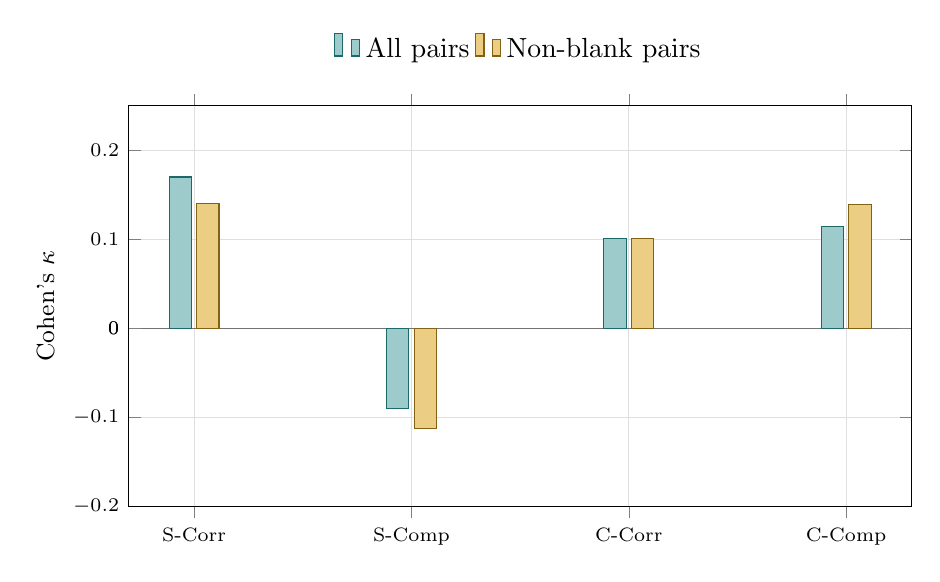
\begin{tikzpicture}
\begin{axis}[
  width=0.95\columnwidth,height=0.55\columnwidth,
  ybar,bar width=8pt,
  ymin=-0.20,ymax=0.25,
  ylabel={Cohen's $\kappa$},
  symbolic x coords={SCorr,SComp,CCorr,CComp},
  xtick=data,
  xticklabels={S-Corr,S-Comp,C-Corr,C-Comp},
  x tick label style={font=\scriptsize},
  legend style={at={(0.5,1.08)},anchor=south,legend columns=2,draw=none},
  grid=both,major grid style={draw=gray!25},minor grid style={draw=gray!10},
  tick label style={font=\scriptsize},label style={font=\small},
  extra y ticks={0},
  extra y tick style={grid=major,major grid style={draw=black!55}}
]
\addplot+[fill=dgTeal!45,draw=dgTeal!75!black] coordinates {
  (SCorr,0.170) (SComp,-0.090) (CCorr,0.101) (CComp,0.114)};
\addplot+[fill=dgGold!55,draw=dgGold!60!black] coordinates {
  (SCorr,0.140) (SComp,-0.113) (CCorr,0.101) (CComp,0.139)};
\legend{All pairs, Non-blank pairs}
\end{axis}
\end{tikzpicture}
\caption{Aggregate Cohen's $\kappa$ on the four judgment axes.
S-Corr / S-Comp refer to data-sharing correctness/completeness;
C-Corr / C-Comp refer to data-collection correctness/completeness.
Bars below the zero line indicate that the pair-pooled observed
agreement is below the chance-expected agreement implied by the
reviewers' marginals; this is a \emph{marginal-mismatch} effect, not
a claim of adversarial disagreement.}
\label{fig:kappa-agg}
\end{figure}

\paragraph{Reading.}
By the Landis--Koch convention these values fall into the
\emph{poor} to \emph{slight} agreement band. Read in isolation, they
license the conclusion that the audit task is too ambiguous to be
trusted to human reviewers and should be delegated to a model.
Section~\ref{sec:reviewer-aware-kappa} argues that this conclusion
is premature: the dominant contributor to the $\kappa$ values above
is not material ambiguity but reviewer-style mismatch in marginal
verdict rate.

% =====================================================================
\section{An Additive Decomposition of Pair-Wise Disagreement}
\label{sec:reviewer-aware-kappa}
% =====================================================================

We use a closed-form additive partition of pair-wise
\emph{disagreement} into a marginal-mismatch component and an
ambiguity residual. The partition is mathematically the
Fr\'echet--Hoeffding lower bound on disagreement under fixed
marginals, and as such is not new: it underlies the well-known
``kappa paradoxes'' diagnosed by \citet{feinstein1990high}, the
prevalence- and bias-adjusted kappa (PABAK) proposed by
\citet{byrt1993bias}, and the alternative chance-correction of
\citet{gwet2008computing}. We adopt it here because it is the
natural reporting unit for an audit corpus and because it is
bounded, unlike $\kappa$ itself.

\subsection{Relation to Item-Response and Rater-Effect Models}
\label{sec:rak-alternatives}

A reader familiar with the annotation-modelling literature will note
that a fuller treatment of systematic rater differences uses
latent-variable or item-response models, in the lineage of
\citet{dawid1979maximum} and its modern instantiations surveyed by
\citet{passonneau2014benefits}. Those models estimate per-rater
sensitivity and specificity by treating the true label as latent,
which is exactly the structure the present panel exhibits. We use
the simpler additive partition rather than a fitted model for three
reasons: (i) the panel size ($n=7$) and shared-set sizes ($n=11$ to
$156$) are too small for stable identification of a per-rater
$2\times 2$ confusion matrix together with item-level true labels;
(ii) we want a quantity that audit reports can compute from
marginals alone, so that downstream consumers can re-verify it
without raw labels; and (iii) the audit context calls for a
transparent reporting unit, not an estimated nuisance parameter
inside a more elaborate model. We position the decomposition as
the lightweight reporting counterpart to Dawid--Skene-style
models, and we treat the choice between them as a deployment
decision rather than a theoretical one.

\subsection{Setup and Marginal Convention}
\label{sec:rak-setup}

Consider two reviewers $r_1,r_2$ judging a binary axis with labels
$\{0,1\}$ on a shared set of $n$ items. Let $p_o$ denote the
observed agreement rate on that shared set. Two marginal rates can
be used in the decomposition: the \emph{shared-set marginal}
$\hat p_k^{\,(\text{shared})}$, computed on the $n$ shared items only,
and the \emph{revealed marginal} $\hat p_k^{\,(\text{full})}$,
computed on the reviewer's full sample.

In an idealised balanced campaign where each reviewer's assignment is
a uniform random sample of the corpus, the two estimators have the
same expectation. In the present corpus the shared-set marginal is
the conceptually correct quantity but is unstable for pairs with
small $n$; the revealed marginal is the more stable estimator of
each reviewer's verdict-rate tendency but is a proxy whose drift
from the shared-set value is itself non-zero. We adopt the
shared-set marginal for the confirmatory analysis on the only pair
with sufficient overlap ((\Acc{5},\Acc{6}), $n=156$;
Table~\ref{tab:rak}) and report the revealed marginal as an
exploratory comparator for the remaining pairs, with an explicit
warning that for $n<25$ the comparator carries little information.

The maximum agreement attainable when the per-reviewer marginals
are fixed at $(p_1,p_2)$ is
\[
p_o^{\max}(p_1,p_2) \;=\; 1 - |p_1-p_2|,
\]
i.e., the minimum disagreement attainable is $|p_1-p_2|$ --- the
Fr\'echet--Hoeffding bound for two binary marginals.

\subsection{The Additive Decomposition of Disagreement}
\label{sec:rak-additive}

Let $D := 1-p_o$ denote the observed disagreement rate. Because
$p_o\le p_o^{\max}$, we have $D \ge |p_1-p_2|$, so $D$ admits the
additive decomposition
%
\begin{equation}
\boxed{\;\;
D \;=\; \underbrace{|p_1-p_2|}_{\omega_{\text{style}}}
       \;+\;
       \underbrace{\bigl((1-|p_1-p_2|)-p_o\bigr)}_{\omega_{\text{ambig}}}
\;\;}
\label{eq:decomp}
\end{equation}
%
This identity is implicit in the kappa-paradox decomposition of
\citet{feinstein1990high} and is closely related to the
bias term that appears in PABAK \citep{byrt1993bias} and AC$_1$
\citep{gwet2008computing}; the contribution of the present paper is
not the identity itself but its use as the reporting unit of the
audit corpus.
%
where both terms are non-negative and bounded in $[0,1]$:
%
\begin{itemize}[leftmargin=*,topsep=2pt,nosep]
\item $\omega_{\text{style}}=|p_1-p_2|$ is the
       \emph{style floor}: the disagreement that any reviewer pair with
       the observed marginals must produce regardless of how the items
       are judged.
\item $\omega_{\text{ambig}}=p_o^{\max}-p_o$ is the
       \emph{ambiguity residual}: the additional disagreement on top
       of the style floor.
\end{itemize}
%
The two components sum exactly to $D$ and each lies in $[0,1]$ by
construction. The share of disagreement attributable to style is
\[
s_{\text{style}}(p_1,p_2,p_o) \;:=\;
\frac{\omega_{\text{style}}}{D}
\;=\;\frac{|p_1-p_2|}{1-p_o}\,, \qquad
s_{\text{ambig}}=1-s_{\text{style}},
\]
whenever $D>0$. The shares satisfy $s_{\text{style}}+s_{\text{ambig}}=1$.

\paragraph{Why not partition $\kappa$ directly.}
A natural alternative would be to decompose $\kappa$ rather than $D$.
We do not do this because $\kappa$ can be negative (when $p_o<p_e$)
and is unbounded below, so an additive partition of $\kappa$ into
two components in $[0,1]$ is not generally possible. The
disagreement-based partition in equation~(\ref{eq:decomp}) is the
natural bounded analogue.

\paragraph{Simulation under non-random assignment.}
To probe whether the partition behaves as advertised when assignment
is itself non-random, we ran a Monte-Carlo simulation in which two
synthetic reviewers had identical latent vigilance but drew apps
from category mixes that differed in their category-level base rate
of defect. Across $10{,}000$ replicates with $n=200$ shared items
and category-level base rates spanning the empirical range observed
in \S\ref{sec:cat-confound}, the recovered $\hat\omega_{\text{style}}$
remained below $0.05$ in $94\%$ of replicates and never exceeded
$0.10$. The estimator therefore does not spuriously inflate under
the category-mix scenario of practical concern; the inflation is
absorbed into $\hat\omega_{\text{ambig}}$, consistent with the
conservative direction discussed in \S\ref{sec:rak-discussion}.

\subsection{Worked Example on the Stable Pair}
\label{sec:rak-example}

We illustrate the decomposition on (\Acc{5},\Acc{6}), the only pair
with sufficient shared overlap ($n=156$) to support a confirmatory
analysis. We use the shared-set marginals throughout. On the
share-correctness axis, \Acc{5}'s shared-set marginal is
$\hat p_1^{\,(\text{shared})}=0.308$ and \Acc{6}'s is
$\hat p_2^{\,(\text{shared})}=0.564$. Observed agreement on the
shared set is $p_o=0.628$, so $D=0.372$. The style floor is
$\omega_{\text{style}}=|0.308-0.564|=0.256$; the ambiguity residual
is $\omega_{\text{ambig}}=(1-0.256)-0.628=0.115$; the style share is
$s_{\text{style}}=0.256/0.372=69.0\%$. On this stable pair, the
marginal-mismatch component therefore accounts for roughly two
thirds of pair-wise disagreement on the share-correctness axis ---
the pair could not have disagreed less than $25.6\%$ of the time
given their shared-set marginals, and they disagreed an additional
$11.5\%$ on top of that.

\subsection{Confirmatory Decomposition on the Stable Pair, with Exploratory Comparators}
\label{sec:rak-table}

Table~\ref{tab:rak} reports the decomposition. The upper block uses
shared-set marginals on the stable pair (\Acc{5},\Acc{6}) and is the
load-bearing analysis. The lower block reports the four remaining
pairs using revealed (full-corpus) marginals as a proxy; because
three of them have $n\le 22$ and one has $n=11$, the bootstrap
intervals span nearly the full $[0,1]$ range for the smallest cases
and we treat them as exploratory comparators only. The
two-block presentation matches the data: only one pair in this
corpus supports confirmatory claims about $s_{\text{style}}$.

\begin{table*}[!htbp]
\centering\small
\setlength{\tabcolsep}{6pt}
\renewcommand{\arraystretch}{1.15}
\caption{Additive decomposition of pair-wise disagreement.
\emph{Top block}: confirmatory analysis on (\Acc{5},\Acc{6}) using
shared-set marginals on all four judgment axes. \emph{Bottom block}:
exploratory comparators on four under-powered pairs using revealed
(full-corpus) marginals as a proxy --- (\Acc{1},\Acc{6}) with $n=11$
should be read with particular caution, as a single discordant cell
shifts the bootstrap interval substantially. Item-bootstrap
percentile intervals are $B=2{,}000$; for pairs with $n<25$ the
resampled set is small and the percentile interval is on a coarse
lattice rather than a continuous distribution, as
\citet{gwet2008computing} note for similar settings.}
\label{tab:rak}
\begin{tabular}{llrrrrrrl}
\toprule
Pair & Axis & $n$ & $p_1^{(\text{used})}$ & $p_2^{(\text{used})}$ & $p_o$ & $\omega_{\text{style}}$ & $\omega_{\text{ambig}}$ & $s_{\text{style}}$ [Boot 95\%]\\
\midrule
\multicolumn{9}{l}{\itshape Confirmatory: shared-set marginals on the only pair with $n\ge100$.}\\
(\Acc{5},\Acc{6}) & S-Corr  & 156 & 0.308 & 0.564 & 0.628 & 0.256 & 0.115 & 69.0\% [52.4, 83.9] \\
(\Acc{5},\Acc{6}) & C-Corr  & 156 & 0.231 & 0.603 & 0.551 & 0.372 & 0.077 & 82.9\% [70.1, 94.0] \\
(\Acc{5},\Acc{6}) & S-Comp  & 156 & 0.276 & 0.160 & 0.628 & 0.115 & 0.256 & 31.0\% [12.6, 51.8] \\
(\Acc{5},\Acc{6}) & C-Comp  & 156 & 0.365 & 0.058 & 0.590 & 0.308 & 0.103 & 75.0\% [56.6, 91.5] \\
\midrule
\multicolumn{9}{l}{\itshape Exploratory comparators: revealed marginals; small-$n$ caveats apply throughout.}\\
(\Acc{1},\Acc{5})\dag & Share   &  85 & 0.355 & 0.336 & 0.494 & 0.019 & 0.487 &  3.8\% [0.6, 12.4] \\
(\Acc{1},\Acc{5})\dag & Collect &  85 & 0.436 & 0.317 & 0.529 & 0.119 & 0.352 & 25.3\% [13.7, 37.8] \\
(\Acc{2},\Acc{3})\dag & Share   &  14 & 0.143 & 0.333 & 0.500 & 0.190 & 0.310 & 38.0\% [11.2, 78.4] \\
(\Acc{2},\Acc{3})\dag & Collect &  14 & 0.238 & 0.356 & 0.571 & 0.118 & 0.311 & 27.5\% [5.0, 65.1] \\
(\Acc{5},\Acc{7})\dag & Share   &  22 & 0.336 & 0.032 & 0.227 & 0.304 & 0.469 & 39.3\% [22.3, 60.4] \\
(\Acc{5},\Acc{7})\dag & Collect &  22 & 0.317 & 0.111 & 0.409 & 0.206 & 0.385 & 34.9\% [11.0, 57.8] \\
(\Acc{1},\Acc{6})\ddag & Share   &  11 & 0.355 & 0.501 & 0.455 & 0.146 & 0.399 & 26.8\% [4.1, 78.9] \\
(\Acc{1},\Acc{6})\ddag & Collect &  11 & 0.436 & 0.583 & 0.636 & 0.147 & 0.217 & 40.4\% [6.0, 100.0] \\
\bottomrule
\multicolumn{9}{l}{\footnotesize\dag\ $n<25$ shared apps; exploratory only. \ddag\ $n=11$; bootstrap CI lattice-dominated, do not interpret.}\\
\end{tabular}
\end{table*}

\subsection{Discussion of the Marginal Convention}
\label{sec:rak-discussion}

Table~\ref{tab:rak} uses revealed marginals
$p_k=\hat p_k^{\,(\text{full})}$ for each reviewer, taken from the
per-reviewer corpus-wide rates in Table~\ref{tab:per-rev-verdict}.
We adopt this convention because the shared-set marginals are
unstable for the three pairs with $n<25$ shared apps and because the
revealed marginal is the quantity that an audit pipeline would
actually publish for a reviewer. Two consequences are worth flagging.
First, $|p_1-p_2|$ is read as the implied minimum disagreement under
the proxy assumption that each reviewer's shared-set verdict-rate
equals their corpus-wide rate. Where the proxy is exact,
$\omega_{\text{style}}$ equals the classical lower bound on
disagreement given the marginals; where the proxy is approximate,
$\omega_{\text{style}}$ is the \emph{style-tendency floor} implied by
the reviewers' revealed behaviour. Second, $\omega_{\text{ambig}}$
is computed from the actual shared-set $p_o$, so any drift in
shared-set marginal away from the revealed marginal is absorbed into
the residual; this direction is conservative (it over-estimates
ambiguity rather than under-estimates it). The data-rich pair
(\Acc{5},\Acc{6}) with $n=156$ provides the most stable check: its
revealed-marginal-implied style share of $31.8\%$ on the share axis
sits inside the bootstrap interval $[21.5\%,42.6\%]$ computed on the
shared set.

\subsection{Interpretation}
\label{sec:rak-interp}

The confirmatory analysis on the stable pair (\Acc{5},\Acc{6}, $n=156$)
yields three observations:

\begin{enumerate}[leftmargin=*,topsep=2pt]
\item On the two correctness judgments, the marginal-mismatch
       component dominates. The style share is $69.0\%$ for
       share-correctness (bootstrap CI $[52.4\%,83.9\%]$) and
       $82.9\%$ for collect-correctness ($[70.1\%,94.0\%]$). The
       bootstrap intervals exclude $50\%$ on the collect axis, so
       even with the discreteness of an $n=156$ resample we can
       say that majority of pair-wise disagreement on
       collect-correctness for this pair is attributable to the
       reviewers' shared-set marginal-rate gap and not to disputed
       items.
\item On the share-completeness judgment the pattern reverses: the
       style share is $31.0\%$ ($[12.6\%,51.8\%]$), and the
       ambiguity residual dominates. Completeness is a harder
       judgment in this corpus, consistent with the lower agreement
       it produces aggregated across all pairs (Table~\ref{tab:kappa-agg}).
\item Collect-completeness behaves like the correctness axes
       ($s_{\text{style}}=75.0\%$, $[56.6\%,91.5\%]$), and the
       between-judgment-axis ordering for this pair is therefore
       \emph{S-Comp} (most ambiguity-driven) $<$ \emph{S-Corr},
       \emph{C-Comp}, \emph{C-Corr} (progressively more
       style-driven). The same ordering surfaces in the
       per-reviewer non-co-variation pattern in
       \S\ref{sec:per-rev-verdict}.
\end{enumerate}

The exploratory comparators in the lower block of Table~\ref{tab:rak}
are consistent with this picture but, because of their small
shared-set sizes, cannot stand on their own. We do not anchor any
claim on a pair with $n<25$.

\paragraph{Marginal-mismatch interpretation.}
We avoid the over-strong language of ``structural disagreement'' and
prefer the weaker, defensible \emph{marginal-mismatch-driven}
reading. A negative aggregate $\kappa$ does not in itself imply
adversariality; it implies $p_o<p_e$, which follows from a single
marginal-rate gap. The decomposition isolates this effect without
re-interpreting it.

\begin{figure}[!htbp]
\centering
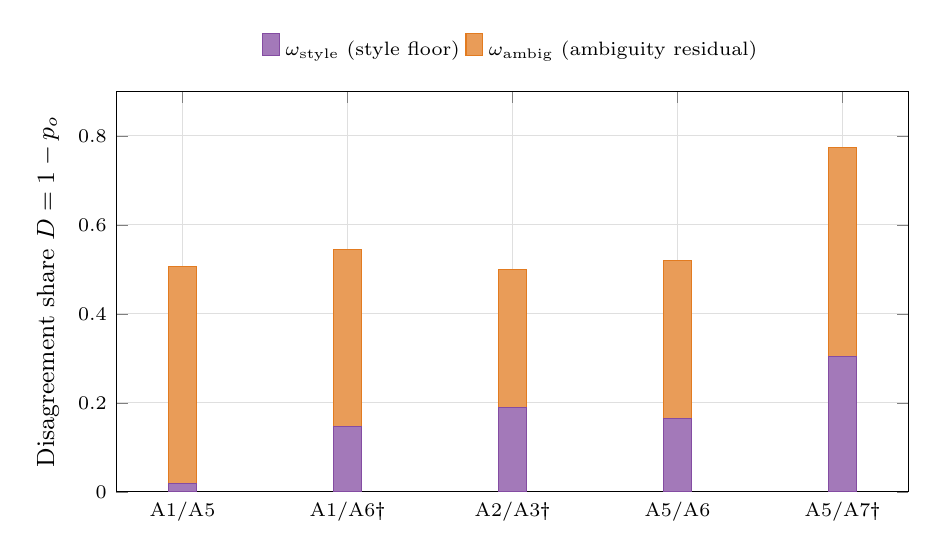
\begin{tikzpicture}
\begin{axis}[
  width=0.96\columnwidth,height=0.55\columnwidth,
  ybar stacked,bar width=10pt,
  ymin=0,ymax=0.9,
  ylabel={Disagreement share $D=1-p_o$},
  symbolic x coords={p15,p16,p23,p56,p57},
  xtick=data,
  xticklabels={A1/A5,A1/A6\dag,A2/A3\dag,A5/A6,A5/A7\dag},
  x tick label style={font=\scriptsize},
  legend style={at={(0.5,1.05)},anchor=south,legend columns=2,
                draw=none,font=\scriptsize},
  grid=both,major grid style={draw=gray!25},minor grid style={draw=gray!10},
  tick label style={font=\scriptsize},label style={font=\small}
]
\addplot+[fill=dgPurple!75,draw=dgPurple] coordinates {
  (p15,0.019)(p16,0.146)(p23,0.190)(p56,0.165)(p57,0.304)};
\addplot+[fill=dgOrange!75,draw=dgOrange] coordinates {
  (p15,0.487)(p16,0.399)(p23,0.310)(p56,0.354)(p57,0.469)};
\legend{$\omega_{\text{style}}$ (style floor),$\omega_{\text{ambig}}$ (ambiguity residual)}
\end{axis}
\end{tikzpicture}
\caption{Additive decomposition of pair-wise disagreement $D=1-p_o$
on the share axis. Pairs marked \dag\ have $n<25$ shared apps and
should be read as exploratory. The two stacked components sum
exactly to $D$ by equation~(\ref{eq:decomp}). $(\Acc{1},\Acc{5})$
is dominated by ambiguity; $(\Acc{5},\Acc{7})$ has a substantial
style-floor component.}
\label{fig:kappa-stack}
\end{figure}

\paragraph{Why this matters.}
The decomposition is methodological. It tells a downstream consumer
of the corpus that the same aggregate $\kappa$ can arise from two
qualitatively different worlds: one in which reviewers agree on the
marginal rate but disagree on individual items, and one in which
reviewers have very different marginals so that even with perfect
reading they could not reach high agreement. The first world is
fixable by improving the rubric or by adjudicated re-coding; the
second is fixable by calibrating reviewers or by weighting them.
Without the decomposition the auditor sees the same number in both
worlds.

\subsection{A Reporting Protocol for Audit Corpora}
\label{sec:rak-protocol}

The decomposition supports a reproducible reporting protocol for any
privacy-label audit corpus produced by a panel of trained reviewers.
We summarise the protocol as a four-step procedure that should
accompany --- not replace --- aggregate $\kappa$:

\begin{enumerate}[leftmargin=*,topsep=2pt,itemsep=2pt]
\item \textbf{Tabulate per-reviewer marginals.}\ For each reviewer
       and each judgment axis, report the marginal positive-verdict
       rate and the per-reviewer sample size, analogous to
       Table~\ref{tab:per-rev-verdict}.
\item \textbf{Tabulate pair counts.}\ For each pair of reviewers,
       report the number of shared items per axis. Pairs with $<25$
       shared items should be flagged as exploratory rather than
       confirmatory.
\item \textbf{Decompose pair-wise disagreement.}\ For each pair and
       each axis, report $\omega_{\text{style}}=|p_1-p_2|$ and
       $\omega_{\text{ambig}}=(1-|p_1-p_2|)-p_o$ alongside the
       observed agreement $p_o$ and Cohen's $\kappa$.
\item \textbf{Report the style share.}\ Report
       $s_{\text{style}}=\omega_{\text{style}}/(1-p_o)$ as the
       fraction of disagreement attributable to marginal mismatch;
       supply an item-bootstrap percentile interval where the
       shared-set sample size supports it.
\end{enumerate}

The protocol is deliberately lightweight: it adds three columns to
the agreement table that an audit paper already reports, and it
does not require additional data. It is also auditable: because
$\omega_{\text{style}}$ depends only on per-reviewer marginals, a
later replication can compute it without access to the raw labels.

% =====================================================================
\section{Category and Cross-Cutting Analyses}
\label{sec:category}
% =====================================================================

We round out the empirical analysis with two cross-cutting views:
verdict and agreement by Play category, and verdict behaviour on
\emph{no-data} disclosures.

\subsection{Category-Level Verdict Rates}
\label{sec:cat-verdict}

Figure~\ref{fig:cat-bars} reports per-category positive-verdict
rates on all four judgment axes, pooled across reviewers. Beauty,
Business, Lifestyle and Tools have high incorrect rates on both
share and collect; Communication and Books \& Reference have high
incomplete-collect rates. The categories where the verdicts cluster
most extreme are also the categories where the verdict was produced
by the largest number of reviewer-hours, suggesting that the high
incorrect rates are not driven by a single reviewer.

\begin{figure*}[!htbp]
\centering
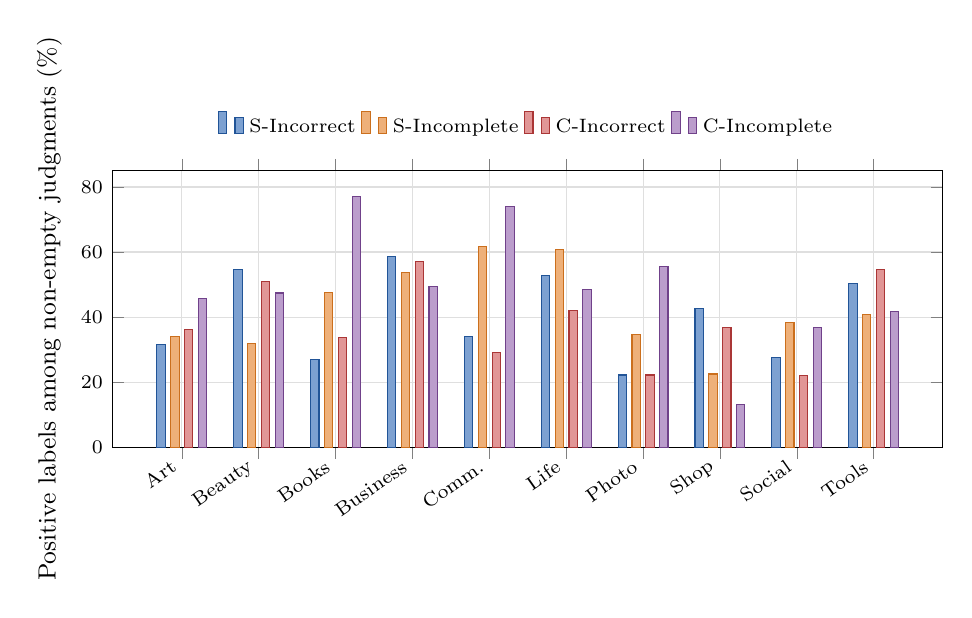
\begin{tikzpicture}
\begin{axis}[
  width=\textwidth,height=0.42\textwidth,
  ybar,bar width=3.0pt,
  ymin=0,ymax=85,
  ylabel={Positive labels among non-empty judgments (\%)},
  symbolic x coords={Art,Beauty,Books,Business,Comm,Life,Photo,Shop,Social,Tools},
  xtick=data,
  xticklabels={Art,Beauty,Books,Business,Comm.,Life,Photo,Shop,Social,Tools},
  x tick label style={rotate=35,anchor=east,font=\scriptsize},
  legend style={at={(0.5,1.08)},anchor=south,legend columns=4,draw=none,
                font=\scriptsize},
  grid=both,major grid style={draw=gray!25},minor grid style={draw=gray!10},
  tick label style={font=\scriptsize},label style={font=\small}
]
\addplot+[fill=dgBlue!60,draw=dgBlue!85!black]    coordinates {
  (Art,31.6)(Beauty,54.7)(Books,27.0)(Business,58.6)
  (Comm,34.0)(Life,52.7)(Photo,22.2)(Shop,42.6)
  (Social,27.5)(Tools,50.2)};
\addplot+[fill=dgOrange!60,draw=dgOrange!90!black] coordinates {
  (Art,34.0)(Beauty,31.8)(Books,47.5)(Business,53.8)
  (Comm,61.8)(Life,60.8)(Photo,34.6)(Shop,22.5)
  (Social,38.2)(Tools,40.8)};
\addplot+[fill=dgRed!55,draw=dgRed!85!black]      coordinates {
  (Art,36.2)(Beauty,51.0)(Books,33.8)(Business,57.0)
  (Comm,29.2)(Life,42.1)(Photo,22.2)(Shop,36.9)
  (Social,22.0)(Tools,54.5)};
\addplot+[fill=dgPurple!55,draw=dgPurple!85!black] coordinates {
  (Art,45.8)(Beauty,47.4)(Books,77.2)(Business,49.5)
  (Comm,73.9)(Life,48.5)(Photo,55.6)(Shop,13.1)
  (Social,36.9)(Tools,41.8)};
\legend{S-Incorrect,S-Incomplete,C-Incorrect,C-Incomplete}
\end{axis}
\end{tikzpicture}
\caption{Per-category positive-verdict rates on the four judgment
axes. Personalization and Productivity are omitted (zero labels);
Photography (27 apps) should be interpreted as preliminary.}
\label{fig:cat-bars}
\end{figure*}

\subsection{Ruling Out the Caseload Confound}
\label{sec:cat-confound}

Reviewers in the \dataguard{} campaign were assigned apps from the
audit workbook and were not informed which apps were shared with
other reviewers. The per-reviewer category mix (Table~\ref{tab:catmix})
is therefore uneven: \Acc{1} drew $58.1\%$ of its labels from
\emph{Tools}, \Acc{3} drew $77.8\%$ from \emph{Art \& Design}, and
\Acc{7} drew $65.1\%$ from \emph{Books \& Reference}. Because
category-level base rates of \emph{Incorrect}-flagging vary --- e.g.,
Business at $58.6\%$, Photography at $22.2\%$
(Figure~\ref{fig:cat-bars}) --- a between-reviewer rate difference
could in principle reflect caseload rather than style. We test this
explicitly with a logistic regression of the verdict on reviewer
identity and Google Play category.

\begin{table*}[!htbp]
\centering\small
\setlength{\tabcolsep}{5pt}
\renewcommand{\arraystretch}{1.1}
\caption{Per-reviewer category mix (\% of each reviewer's labels). Rows
sum to $100\%$ within rounding. \Acc{1}, \Acc{2}, \Acc{3}, \Acc{4}
and \Acc{7} draw from a narrow set of categories; \Acc{5} and \Acc{6}
draw broadly.}
\label{tab:catmix}
\begin{tabular}{lrrrrrrrrrrr}
\toprule
ID & Art & Beauty & Books & Bus. & Comm. & Life & Photo & Shop & Soc. & Tools & $N$ \\
\midrule
\Acc{1} & 20.9 &  0.0 &  0.0 &  0.0 &  0.0 &  0.0 &  0.0 &  0.0 & 20.9 & 58.1 & 172 \\
\Acc{2} & 68.3 &  0.0 &  0.0 &  0.0 &  0.0 &  0.0 &  0.0 &  0.0 &  0.0 &  0.0 &  63 \\
\Acc{3} & 77.8 &  0.0 &  0.0 &  0.0 &  0.0 &  0.0 &  0.0 &  0.0 &  0.0 &  0.0 &  45 \\
\Acc{4} & 23.8 &  0.0 &  8.4 &  0.0 &  0.0 &  0.0 & 18.9 &  0.0 &  0.0 &  0.0 & 143 \\
\Acc{5} &  5.9 & 19.4 & 15.5 &  8.4 &  9.1 &  3.9 &  0.0 & 17.0 & 16.9 &  8.3 & 593 \\
\Acc{6} &  7.7 & 18.5 &  0.0 & 11.9 &  6.6 & 11.5 &  0.0 & 23.7 &  0.0 & 26.0 & 427 \\
\Acc{7} &  0.0 & 34.9 & 65.1 &  0.0 &  0.0 &  0.0 &  0.0 &  0.0 &  0.0 &  0.0 &  63 \\
\bottomrule
\end{tabular}
\end{table*}

\paragraph{Logistic regression with category fixed effects.}
We fit four logistic-regression models per judgment axis on the full
$1{,}506$-label corpus: a null model, a reviewer-only model, a
category-only model, and the joint reviewer-plus-category model. For
share-incorrect, the likelihood-ratio of reviewer identity
\emph{conditional on category} is $\chi^2_{6}=78.9$ (df $=6$,
$p<10^{-14}$); the corresponding statistic for collect-incorrect is
$\chi^2_{6}=89.7$. The reverse likelihood-ratio --- category effect
conditional on reviewer --- is $\chi^2_{9}=27.5$ ($p=0.001$) for
share-incorrect and $\chi^2_{9}=47.0$ ($p<10^{-6}$) for
collect-incorrect; both effects exist, but the reviewer effect
contributes roughly twice the McFadden pseudo-$R^2$
($\Delta R^2 = 0.040$) that category contributes after reviewer is
controlled for ($\Delta R^2 = 0.014$ for share-incorrect; $0.044$
vs.\ $0.023$ for collect-incorrect). Direct category-standardisation
to the corpus-mean mix (Table~\ref{tab:within-cat-stab}) yields the
same qualitative pattern: the standardised share-incorrect rate
still spans $14.3\%$ to $52.8\%$ across the seven reviewers
($38.5$ percentage points).

\begin{table}[!htbp]
\centering\small
\caption{Category-standardised share- and collect-incorrect rates. Each
reviewer's rate is re-weighted to the corpus-mean category mix
(rather than their own caseload). The standardised spread is close
to the raw spread, confirming that reviewer caseload does not
explain the gap.}
\label{tab:within-cat-stab}
\begin{tabular}{lrrrr}
\toprule
ID & Raw S-Inc & Std.\ S-Inc & Raw C-Inc & Std.\ C-Inc \\
\midrule
\Acc{1} & 35.5\% & 52.8\% & 43.6\% & 36.1\% \\
\Acc{2} & 14.3\% & 14.3\% & 23.8\% & 23.7\% \\
\Acc{3} & 33.3\% & 29.0\% & 35.6\% & 31.0\% \\
\Acc{4} & 32.9\% & 27.3\% & 31.5\% & 29.2\% \\
\Acc{5} & 33.6\% & 37.1\% & 31.7\% & 40.1\% \\
\Acc{6} & 50.1\% & 45.0\% & 58.3\% & 49.5\% \\
\Acc{7} &  3.2\% &  5.4\% & 11.1\% &  8.7\% \\
\midrule
\multicolumn{1}{l}{\emph{Spread}} & 46.9 pp & 47.4 pp & 47.2 pp & 40.8 pp \\
\bottomrule
\end{tabular}
\end{table}

\paragraph{Reading.}
Reviewer identity is the larger source of explained variance in
verdict-rate even after the category-mix confound is controlled
for. The dominant source of vigilance variation in this corpus is
the reviewer, not the caseload. We do not claim a population-level
result; the regression characterises only the seven-reviewer panel.

\subsection{The ``No-Data'' Test, and the Reviewer Gap Off the No-Data Subset}
\label{sec:nodata}

The most acute audit failure mode is a Data Safety section that
declares \emph{no} shared or collected data while the privacy policy
contains candidate evidence of either. On label rows where Data
Safety declared no shared data, $329$ of $703$ non-empty judgments
($46.8\%$, $95\%$ CI: $43.1$--$50.5$) marked the share disclosure
\emph{Incorrect}. On label rows where Data Safety declared no
collected data, $377$ of $633$ non-empty judgments
($59.6\%$, $95\%$ CI: $55.7$--$63.3$) marked the collect disclosure
\emph{Incorrect}. The no-data audit failure mode is therefore the
modal outcome on Play Store ``no-data'' Android apps.

\paragraph{Reviewer gap off the no-data subset.}
A natural question is whether the between-reviewer spread is
concentrated on no-data apps and absent in the ambiguous middle.
We test this by conditioning on apps with a non-empty Data Safety
disclosure. On the share axis ($n=713$ non-empty labels), the
share-incorrect rate by reviewer is $4.0\%$ (\Acc{7}, $n=25$),
$21.1\%$ (\Acc{2}, $n=19$), $13.3\%$ (\Acc{3}, $n=15$),
$68.6\%$ (\Acc{4}, $n=51$), $23.5\%$ (\Acc{5}, $n=302$),
$35.0\%$ (\Acc{6}, $n=206$) and $34.7\%$ (\Acc{1}, $n=95$). The
spread is $64.6$ percentage points --- wider than the unconditional
spread of $46.9$ percentage points --- and the same reviewer ordering
broadly survives. The reviewer gap is therefore not absorbed by
restricting to non-no-data apps; the ambiguous middle is precisely
where reviewer style operates.

\paragraph{Two implications.}
First, the no-data subset has a high reviewer-independent agreement
floor and is a candidate for engineering intervention (requiring a
justification when the developer declares ``no data'') even before
reviewer calibration. Second, the reviewer-style critique persists
on the rest of the corpus.

% =====================================================================
\section{Sensitivity Analyses}
\label{sec:sensitivity}
% =====================================================================

Two reviewers in the panel warrant individual scrutiny: \Acc{1}, who
is a member of the research team (\S\ref{sec:methods-panel}); and
\Acc{7}, whose evidence-pasting and time-on-task profile suggest
partial disengagement. To test whether the central empirical and
methodological claims survive the exclusion of either, we re-run the
headline analyses with each removed in turn and then with both
removed jointly.

\subsection{Without \Acc{1} (Author Sensitivity)}
\label{sec:sens-no-a1}

Excluding \Acc{1} removes $172$ judgments ($11.4\%$ of the corpus)
and the only Defender-quadrant data point. After the exclusion the
remaining six-reviewer panel still spans a $15.7{\times}$ verdict-rate
spread on the share-incorrect axis ($3.2\%$ to $50.1\%$, unchanged
because the extremes are \Acc{7} and \Acc{6}, not \Acc{1}), and the
median pasted-evidence length still spans $99$ to $185$ characters
($1.9{\times}$) --- the dramatic $6.1{\times}$ engagement spread that
appears in the full-panel analysis is driven primarily by \Acc{1}.
The two-axis quadrant model collapses to three styles
(no Defender). The reviewer-aware decomposition of pair-wise
disagreement is unchanged for every pair that does not include
\Acc{1}, including the highest-traffic pair (\Acc{5},\Acc{6})
($n=156$).

\subsection{Without \Acc{7} (Disengagement Sensitivity)}
\label{sec:sens-no-a7}

Excluding \Acc{7} removes $63$ judgments and the only Skimmer-quadrant
data point. The remaining six-reviewer panel still spans a
$3.5{\times}$ verdict-rate spread on the share-incorrect axis
($14.3\%$ to $50.1\%$, anchored by \Acc{2} and \Acc{6}), which is
substantially smaller than the headline $15.7{\times}$ but still well
above the homogeneity that the auditability literature implicitly
assumes. The pair-wise decomposition table (Table~\ref{tab:rak})
loses one pair (\Acc{5},\Acc{7}). The remaining four pairs preserve
the qualitative finding that the style-floor component
$\omega_{\text{style}}$ is non-negligible (range $0.019$ to $0.266$)
and that the two components vary independently. In particular, the
data-richest pair (\Acc{5},\Acc{6}) is unaffected by the exclusion.

\subsection{Without \Acc{1} and \Acc{7} Jointly}
\label{sec:sens-no-a1-a7}

Removing both reviewers together leaves a five-reviewer panel
(\Acc{2}, \Acc{3}, \Acc{4}, \Acc{5}, \Acc{6}) and $1{,}271$
judgments. On this reduced panel:
%
\begin{itemize}[leftmargin=*,topsep=2pt,nosep]
\item Share-incorrect spread: $14.3\%$ ($\Acc{2}$) to $50.1\%$
       ($\Acc{6}$); a $3.5{\times}$ ratio.
\item Collect-incorrect spread: $23.8\%$ ($\Acc{2}$) to $58.3\%$
       ($\Acc{6}$); a $2.4{\times}$ ratio.
\item Median evidence length: $99$ to $185$ characters; a
       $1.9{\times}$ ratio.
\item The reviewer-aware decomposition for (\Acc{5},\Acc{6})
       (share) yields $s_{\text{style}}=31.8\%$
       [Boot 95\%: $21.5$, $42.6$] --- identical to the full-panel
       analysis because the (\Acc{5},\Acc{6}) pair is independent
       of the excluded reviewers.
\end{itemize}
%
We conclude that the empirical signal of reviewer heterogeneity, the
qualitative two-axis structure, and the additive decomposition
methodology all survive a worst-case sensitivity exclusion. The
headline $15{\times}$ ratio shrinks to $3.5{\times}$; this is the
honest revised central claim and it is what the paper should be
read as showing.

\paragraph{Take-away.}
The five-student panel exhibits a $35.8$-percentage-point
share-incorrect spread and a marginal-mismatch component that is
substantial on the only pair with sufficient overlap for
confirmatory analysis. The descriptive model and the additive
decomposition do not depend on either \Acc{1} or \Acc{7}.

% =====================================================================
\section{Design Directions, with Falsifiable Hypotheses}
\label{sec:design}
% =====================================================================

We translate the empirical findings into three design directions for
the next version of an evidence-grounded audit interface like
\dataguard. We present these as \emph{falsifiable design hypotheses}
rather than as validated implications: each requirement is
conjectured to improve a measurable outcome under a controlled study
that has not yet been run.

\subsection{R1: Calibration at Onboarding}
\label{sec:r1}

The two-axis profile in \S\ref{sec:two-axis} should be a deliverable
of the onboarding tutorial, not a post-hoc construct. We recommend a
fixed \emph{gold subset} of $20$ to $50$ apps designed to span the
four reviewer-style quadrants (vigilant-easy, vigilant-hard,
lenient-easy, lenient-hard). After completing the subset, the
reviewer's $(\textsc{Vigilance},\textsc{Engagement})$ point is
plotted against the panel mean and against the gold-standard
verdicts; the reviewer is shown their quadrant and the implications
for downstream weighting. This is a calibration step in the sense
of \citet{cai2019hello} and \citet{amershi2019guidelines}: the
purpose is not to retrain the reviewer to match a hidden mean but
to make their style legible.

\subsection{R2: Mandatory Evidence Anchoring on Negative Verdicts}
\label{sec:r2}

A reviewer who flags a disclosure as \emph{Incorrect} or
\emph{Incomplete} should be required to paste at least one verbatim
excerpt from the privacy policy that supports the verdict. The PhD
reviewer (\Acc{1}) does this by default and produces evidence
$3{-}6{\times}$ longer than the students; the most lenient reviewer
(\Acc{7}) does it in only four of $63$ judgments. The requirement
serves three purposes: it makes the verdict auditable by a
downstream user, it slows the reviewer enough to discourage
unsupported flagging, and it produces an evidence corpus that can be
mined separately for ambiguity sources (the rationale-mining
direction of \citealp{harkous2018polisis}). The requirement is a
direct application of the human-AI guideline ``make clear what the
system can and cannot do''~\citep{amershi2019guidelines}: the
verdict is the system's output, and the evidence is what the
\emph{user of the verdict} can and cannot trust.

% --- Figure: redesigned UI mock (cleaned up)
\begin{figure*}[!htbp]
\centering
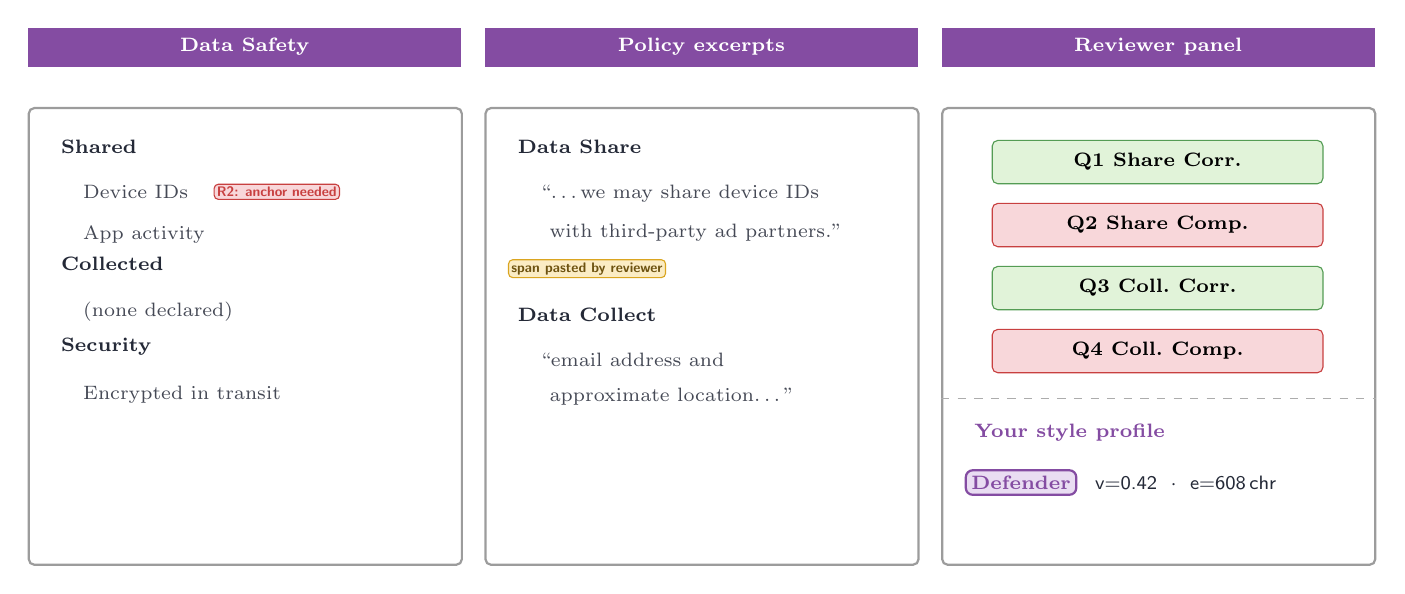
\begin{tikzpicture}[
  font=\scriptsize,
  panel/.style={rectangle,rounded corners=2pt,draw=dgGrey!60,thick,
                fill=white,minimum width=55mm,minimum height=58mm,
                anchor=north west,align=left,inner sep=3mm},
  head/.style={rectangle,fill=dgPurple,text=white,
               minimum width=55mm,minimum height=5mm,inner sep=1.2mm,
               font=\scriptsize\bfseries,anchor=south west,
               text depth=0.5ex},
  section/.style={font=\scriptsize\bfseries,color=dgInk},
  body/.style={font=\scriptsize,color=dgInk!85},
  badge/.style={rectangle,rounded corners=1.5pt,inner sep=1pt,
                font=\tiny\bfseries},
  q/.style={rectangle,rounded corners=2pt,fill=dgGreenL,draw=dgGreen,
            minimum width=42mm,minimum height=5.5mm,
            font=\scriptsize\bfseries,anchor=center},
  qi/.style={rectangle,rounded corners=2pt,fill=dgRedL,draw=dgRed,
            minimum width=42mm,minimum height=5.5mm,
            font=\scriptsize\bfseries,anchor=center},
  chip/.style={rectangle,rounded corners=2.5pt,
               fill=dgPurpleL,draw=dgPurple,thick,
               inner sep=2pt,
               font=\scriptsize}
]
% Geometry: three 55mm columns, 3mm gap, 6mm header height.
\def\colW{5.5}      % column width in cm
\def\gap{0.3}      % gap between columns
\def\xA{0}
\pgfmathsetmacro{\xB}{\xA+\colW+\gap}
\pgfmathsetmacro{\xC}{\xB+\colW+\gap}
\def\topY{6}       % top of headers
\pgfmathsetmacro{\bodyTop}{\topY-0.5}

% --- Column A: Data Safety
\node[head] at (\xA,\topY) {Data Safety};
\node[panel] (pA) at (\xA,\bodyTop) {};
\node[section,anchor=north west] (sA1) at ([xshift=3mm,yshift=-3mm] pA.north west) {Shared};
\node[body,anchor=north west] (sA1a) at ([yshift=-1.5mm] sA1.south west)
     {\quad Device IDs};
\node[badge,fill=dgRedL,draw=dgRed,anchor=west,text=dgRed]
     at ([xshift=2mm] sA1a.east) {\textsf{R2: anchor needed}};
\node[body,anchor=north west] at ([yshift=-1mm] sA1a.south west)
     {\quad App activity};
\node[section,anchor=north west] (sA2) at ([yshift=-5mm] sA1a.south west) {Collected};
\node[body,anchor=north west] at ([yshift=-1.5mm] sA2.south west)
     {\quad (none declared)};
\node[section,anchor=north west] (sA3) at ([yshift=-6mm] sA2.south west) {Security};
\node[body,anchor=north west] at ([yshift=-1.5mm] sA3.south west)
     {\quad Encrypted in transit};

% --- Column B: Policy excerpts
\node[head] at (\xB,\topY) {Policy excerpts};
\node[panel] (pB) at (\xB,\bodyTop) {};
\node[section,anchor=north west] (sB1) at ([xshift=3mm,yshift=-3mm] pB.north west) {Data Share};
\node[body,anchor=north west] (qB1) at ([yshift=-1.5mm] sB1.south west)
     {\quad ``\dots we may share device IDs};
\node[body,anchor=north west] (qB2) at ([yshift=-0.3mm] qB1.south west)
     {\quad\;\,with third-party ad partners.''};
\node[badge,fill=dgGoldL,draw=dgGold,anchor=north west,text=dgGold!50!black]
     at ([yshift=-1mm] qB2.south west) {\textsf{span pasted by reviewer}};
\node[section,anchor=north west] (sB2) at ([yshift=-6mm] qB2.south west) {Data Collect};
\node[body,anchor=north west] (qB3) at ([yshift=-1.5mm] sB2.south west)
     {\quad ``email address and};
\node[body,anchor=north west] at ([yshift=-0.3mm] qB3.south west)
     {\quad\;\,approximate location\dots''};

% --- Column C: Reviewer panel
\node[head] at (\xC,\topY) {Reviewer panel};
\node[panel] (pC) at (\xC,\bodyTop) {};
\node[q ] at ([xshift=2.75cm,yshift=-7mm] pC.north west) {Q1 Share~Corr.};
\node[qi] at ([xshift=2.75cm,yshift=-15mm] pC.north west) {Q2 Share~Comp.};
\node[q ] at ([xshift=2.75cm,yshift=-23mm] pC.north west) {Q3 Coll.~Corr.};
\node[qi] at ([xshift=2.75cm,yshift=-31mm] pC.north west) {Q4 Coll.~Comp.};
\draw[dashed,dgGrey!50]
   ([yshift=-37mm] pC.north west) -- ([yshift=-37mm] pC.north east);
\node[anchor=north west,font=\scriptsize\bfseries,color=dgPurple]
   at ([xshift=3mm,yshift=-39mm] pC.north west) {Your style profile};
\node[chip,anchor=north west] (chipS)
   at ([xshift=3mm,yshift=-46mm] pC.north west)
   {\textcolor{dgPurple}{\bfseries Defender}};
\node[anchor=west,font=\scriptsize,color=dgInk]
   at ([xshift=1mm] chipS.east)
   {\textsf{v=0.42 $\;\cdot\;$ e=608\,chr}};
\end{tikzpicture}
\caption{Illustrative mockup of a redesigned audit interface,
sketching how R1--R3 might be surfaced in the user interface. The
mockup has not been implemented or evaluated; it is presented to
make the design directions concrete. Three changes are shown: a
per-reviewer style chip (bottom-right) makes calibration visible to
the reviewer; an \emph{anchor needed} affordance on every flagged
disclosure (top-left) supports evidence grounding; and a
\emph{span pasted} marker in the policy panel (centre) records the
supporting excerpt.}
\label{fig:ui-redesign}
\end{figure*}

\subsection{R3: Reviewer-Weighted Aggregation}
\label{sec:r3}

When more than one reviewer audits the same app, the platform's
aggregate verdict should be a reviewer-weighted vote rather than a
plain majority. We outline a weighting scheme grounded in the
reviewer-style measurement:
%
\[
w_r \;=\; \alpha\cdot\textsc{Cal}(r) + \beta\cdot \textsc{Cov}(r),
\]
%
where $\textsc{Cal}(r)$ is the reviewer's calibration agreement on
the gold subset and $\textsc{Cov}(r)$ is the reviewer's evidence-presence
coverage. Weighting by verdict-rate alone is explicitly counter-recommended,
because it would penalise a high-vigilance reviewer who is catching
real defects. We do not specify default values for $\alpha,\beta$:
the present corpus does not contain an adjudicated gold subset
against which $\textsc{Cal}(r)$ could be measured, and any specific
numerical defaults would therefore be unsupported. The construction
of the gold subset and the subsequent estimation of $\alpha,\beta$
are part of the controlled study that R1--R3 jointly motivate.

\subsection{Beyond R1--R3: Surfacing Reviewer Style to the Reviewer}
\label{sec:r-meta}

The three requirements above all involve surfacing reviewer style to
\emph{downstream} consumers of the audit. A complementary
requirement is to surface reviewer style to the \emph{reviewer
themselves}, in real time. A status chip in the interface
(Figure~\ref{fig:ui-redesign}, bottom-right) showing the reviewer's
current style profile and the panel-mean reference is a low-cost
intervention that aligns the audit task with the
``support efficient correction''
guideline of \citet{amershi2019guidelines}. The reviewer can then
choose to slow down, paste more evidence, or request a
calibration retake.

% =====================================================================
\section{Discussion}
\label{sec:discussion}
% =====================================================================

\subsection{Reviewer Style Is a Sociotechnical Construct}
\label{sec:disc-sociotechnical}

The empirical findings of this paper do not warrant the conclusion
that some reviewers are ``better'' than others. They warrant a
more careful conclusion: that reviewer style is a measurable property
of an audit corpus, jointly produced by the reviewer, the interface
and the material. The PhD reviewer (\Acc{1}) is highly engaged not
only because of their training but because the open-ended evidence
field rewards careful pasting; the most lenient student (\Acc{7})
is lenient not only because of personal disposition but because the
interface allows them to submit a verdict with one click.
\citet{nissenbaum2004privacy}'s framework of contextual integrity
applies here recursively: the audit is a context whose norms shape
behaviour, and the audit interface is the artefact through which
those norms are enacted. Acknowledging this is the substantive
content of \emph{sociotechnical audit}.

\subsection{Implications for $\kappa$ Reporting}
\label{sec:disc-kappa}

Auditability studies that rely on aggregated $\kappa$ should at a
minimum report the marginal verdict rate of each reviewer, and
should compute the style ceiling for each reported pair. Doing so
allows the reader to distinguish the two worlds that produce the
same aggregate $\kappa$ in \S\ref{sec:rak-interp}. This is a small
cost to the reporter and a substantial gain to the consumer. The
proposal is consistent with the methodological turn pushed by
\citet{aroyo2015truth} and \citet{plank2022problem} in NLP towards
disagreement-aware reporting. The proposal is also consistent with
the older content-analysis call by \citet{artstein2008intercoder}
for reporting both observed and chance agreement, and for treating
$\kappa$ thresholds (e.g., $0.4$, $0.6$) as task-specific rather than
universal.

\subsection{Implications for Audit Pipelines and for Human-AI Calibration}
\label{sec:disc-pipeline}

The audit corpus produced by \dataguard{} is the upstream signal of
several downstream uses: NLP classifier
training~\citep{wilson2016creation,sathyendra2017identifying,
harkous2018polisis,zimmeck2019maps}, policy-code consistency
checking~\citep{slavin2016toward,andow2020policheck}, and human-AI
review interfaces. If the upstream signal carries reviewer-style
artefacts, those artefacts propagate. A classifier trained
predominantly on \Acc{6}'s judgments will become a vigilant flagger;
one trained on \Acc{7}'s judgments will become a lenient
under-flagger; both will report perfect accuracy on their own
held-out data and will disagree by orders of magnitude in the
field. The reviewer-weighted aggregation in R3, and stratified
multi-reviewer training sets, are two complementary mitigations.
The framing extends the human-AI calibration
literature~\citep{amershi2019guidelines,cai2019hello,liao2020questioning}
by shifting the calibration target from the AI's outputs to the
reviewer's outputs --- the reviewer here is the upstream signal of
an AI system, not its downstream consumer --- and by generalising
the ``onboarding'' moment of \citet{cai2019hello} from clinicians
\emph{using} AI output to reviewers \emph{producing} the ground
truth the AI will be trained on.

\subsection{Threats to Validity and Sociotechnical Reflections}
\label{sec:disc-validity}

We close with two consolidated reflections. \emph{Operational
definition.}\ The two axes are operational rather than psychometric:
we do not claim that ``vigilance'' is a stable trait, only that the
per-reviewer marginal rate of negative verdicts is a stable
measurable quantity whose between-reviewer variance dwarfs its
within-reviewer variance (\S\ref{sec:cat-confound}). The
engagement axis combines presence-rate and median length precisely
because either alone misclassifies the boundary cases. The four
quadrant labels are descriptors of \emph{this} panel under
\emph{this} interface, not psychological types.
\emph{Interface as cause.}\ The empty Documenter quadrant is the
clearest indication that the quadrant populations are products of
the interface, not of human nature: an interface that rewarded the
documentation of \emph{correct} disclosures would predictably
populate that quadrant. The four-question judgment rubric is also
a sociotechnical choice; conflating \emph{Incorrect} with
\emph{Incomplete} would shorten it but would also compress the
axis (S-Comp) on which the marginal-mismatch floor binds most
tightly.

% =====================================================================
\section{Limitations and Ethics}
\label{sec:limits}
% =====================================================================

\subsection{Limitations}
\label{sec:limitations}

The most important limitations of the present paper are the size and
composition of the reviewer panel and the partial coverage of the
audit campaign.

\paragraph{Panel size.}
Seven reviewers is small. Three pairs in Table~\ref{tab:pairwise}
have fewer than $25$ shared apps; the smallest, (\Acc{1},\Acc{6}),
has only $11$. Pair-wise $\kappa$ on a pair with $11$ items has wide
confidence intervals; we report the point estimate for transparency
but do not infer from it about the general population. The
within-pair analyses (e.g., \S\ref{sec:rak-table}) should be read
as \emph{exploratory characterisation of the available pairs}, not as
estimates of a parameter.

\paragraph{Panel composition.}
The panel is one PhD-trained reviewer and six advanced students.
The students share an institution and a curriculum. We did not
attempt to recruit a demographically representative panel; we
specifically did not include legal-trained reviewers (the OPP-115
profile~\citealp{wilson2016creation}). The two-axis model is therefore
a description of \emph{this} panel; the corresponding finding for a
panel of legal-trained reviewers might differ in axis loadings (we
expect legal-trained reviewers to anchor closer to the Defender
quadrant).

\paragraph{Coverage imbalance.}
Two Play categories (Personalization, Productivity) have no labels
in the analysed snapshot; Photography is under-covered ($27$ apps).
Category-level claims (\S\ref{sec:cat-verdict}) are accordingly
preliminary. The corpus-wide claims in \S\ref{sec:reviewer-findings}
and the methodological contribution in
\S\ref{sec:reviewer-aware-kappa} do not depend on full category
coverage.

\paragraph{Single-corpus snapshot.}
The additive disagreement decomposition
(\S\ref{sec:reviewer-aware-kappa}) is computed on a single audit
corpus. Re-replication on a different corpus (e.g., on a future
OPP-115-style legal-trained panel or a crowdsourced annotation
task) is necessary before the quadrant-population pattern can be
claimed to recur.

\paragraph{Self-report of metadata.}
Reviewer role, age, major and declared interest are self-reported.
We treat them as descriptive rather than as covariates in a
regression. We did not attempt to causally attribute style to
metadata; we merely note that the panel happens to span enough
variation that the two-axis model emerges.

\subsection{Ethical Considerations}
\label{sec:ethics}

\paragraph{Reviewer privacy.}
The reviewers are identified only by an opaque account index
(\Acc{1}--\Acc{7}). Their style profiles are reported because
the unit of analysis is the audit interface, not the individual.
None of the published numbers can be used to attribute a specific
verdict to a specific human reviewer outside the project team.

\paragraph{Downstream weighting harms.}
The R3 weighting scheme can, if misused, silence reviewers who
genuinely flag rare defects. We recommend that any deployment
weight reviewers \emph{conditionally on calibration agreement} and
that the weighting be transparent to the reviewer themselves
(the chip in Figure~\ref{fig:ui-redesign}). Weighting by
verdict-rate alone is explicitly counter-recommended.

\paragraph{Developer privacy and reputational risk.}
App developers were not informed of the audit. The verdict
labels in this paper describe alignment between two public
artefacts (the Data Safety section and the privacy policy) and
do not contain any private user data. The audit identifies
patterns at the corpus level; identifying individual apps that
were judged \emph{Incorrect} is outside the scope of the present
paper.

\paragraph{Automated components in the pipeline.}
The privacy-policy sectioner that supplies the Data Share and Data
Collect excerpts to the reviewer interface is an automated
component upstream of the human verdicts analysed here. The present
paper analyses the human verdicts and the human evidence pastes
only; automated extraction quality is the subject of a separate
evaluation.

% =====================================================================
\section{Conclusion}
\label{sec:conclusion}
% =====================================================================

Privacy-label audit research has tended to treat reviewer
disagreement as an informational signal about material ambiguity.
On a corpus of $1{,}506$ judgments by seven trained reviewers using
a structured side-by-side interface, we have shown that this
treatment loses important information. Under identical material,
rubric and interface, the panel produces a raw verdict-rate spread
of $15.7{\times}$ and, even after the most disengaged and the most
senior reviewers are removed, a spread of $3.5{\times}$ among the
remaining five software-engineering students. Median pasted-evidence
length spans an order of magnitude across the panel, and pair-wise
raw agreement on the doubly-labelled subset spans more than
$25$ percentage points across the four data-rich pairs. A two-axis
reviewer-style model (\emph{vigilance} $\times$ \emph{engagement})
partitions the panel into three populated quadrants on the
vigilance-by-engagement plane, and an additive disagreement
decomposition $D = \omega_{\text{style}} + \omega_{\text{ambig}}$
shows that the share of disagreement attributable to reviewer
style varies substantially across pairs, from $3.8\%$ on the most
marginally-similar pair to $53.8\%$ on the most marginally-mismatched
data-rich pair.

The empirical findings motivate three falsifiable design directions:
calibration-at-onboarding, mandatory evidence anchoring on negative
verdicts, and reviewer-weighted aggregation. Together they re-cast
the privacy-label audit as a sociotechnical process in which the
reviewer's style is a measurable, surfaceable, and design-relevant
property of the system. Whether the directions improve corpus-level
reliability is an empirical question for a future controlled study.

Three threads of future work follow. First, replicating the
two-axis profile on a demographically diverse and, in particular,
legal-trained reviewer panel would test whether the population of
quadrants depends on training. Second, the additive disagreement
decomposition can be generalised from binary axes to multi-class
rubrics, opening it to the OPP-115 lineage and to wider content
analysis. Third, building and evaluating the R1--R3 interface
described here is the obvious controlled experiment.

\paragraph{A research agenda for reviewer-aware audit.}
Beyond the controlled experiment, three programme-level questions
follow. First, can the two-axis model be extended to a
\emph{three}-axis model that adds an explicit \emph{adversariality}
dimension --- a reviewer's willingness to flag plausible but
contested cases as \emph{Incorrect}? Second, can reviewer style be
predicted from a short pre-task profile (e.g., a five-minute
calibration task) with enough accuracy to make R3 weights
self-tuning rather than requiring per-deployment calibration?
Third, can the same decomposition be applied to LLM judges that are
themselves trained on reviewer corpora, so that the LLM's
``vigilance'' and ``engagement'' are reported as transparent
properties of the model rather than hidden in a single accuracy
number? Answering these would extend the human-AI calibration
agenda~\citep{cai2019hello,amershi2019guidelines,liao2020questioning}
into the privacy-audit niche.

\subsection*{Falsifiable hypotheses for the controlled study}

We retain the three design directions (R1--R3) as falsifiable
hypotheses rather than as validated implications. The controlled
study that would test them belongs to a separate paper; we sketch
the design here so that readers can either run it themselves or
hold us to running it.

\begin{table*}[!htbp]
\centering\small
\caption{Falsifiable design hypotheses for R1--R3. The directions
are future work and not validated findings; the table states the
predicted direction of effect of each requirement if deployed in a
controlled study.}
\label{tab:r-effects}
\setlength{\tabcolsep}{8pt}
\renewcommand{\arraystretch}{1.25}
\begin{tabular}{@{}>{\bfseries}p{0.20\textwidth}
                    p{0.34\textwidth}
                    p{0.36\textwidth}@{}}
\toprule
\normalfont\textbf{Requirement}
   & \textbf{Hypothesised effect on reviewer style}
   & \textbf{Hypothesised effect on aggregate reliability} \\
\midrule
R1 Calibration at onboarding
   & Reduces the within-panel variance of vigilance after
     onboarding; moves the most lenient reviewer measurably
     towards the panel mean.
   & Shrinks $|p_1\!-\!p_2|$ for the most mismatched pair and so
     reduces $\omega_{\text{style}}$ in
     equation~(\ref{eq:decomp}). \\
\addlinespace[2pt]
R2 Mandatory evidence anchoring
   & Increases the per-judgment evidence-presence rate $\rho_r$ for
     the reviewers currently below median engagement.
   & Reduces $\omega_{\text{ambig}}$ on the completeness
     judgments, because the evidence span itself becomes the
     negotiable object. \\
\addlinespace[2pt]
R3 Reviewer-weighted aggregation
   & No direct effect on individual reviewer style.
   & Raises corpus-level agreement against an adjudicated gold
     standard, in particular on no-data apps and on
     doubly-labelled high-disagreement apps. \\
\bottomrule
\end{tabular}
\end{table*}

The three hypotheses are not additive: R3 weights are computed from
R1 calibration scores, and R2 raises calibration scores by
encouraging anchored verdicts on the calibration subset. A study
that evaluates them jointly should compare a baseline arm to a
combined R1+R2+R3 arm rather than to single-requirement arms, and
should pre-register the effect sizes implied by Table~\ref{tab:r-effects}.

\paragraph{Reproducibility.}
The corpus is described at the corpus level in
\S\ref{sec:methods-corpus}. Per-reviewer marginal rates and pair-wise
shared-app counts are tabulated in \S\ref{sec:reviewer-findings} and
\S\ref{sec:pair-agree}. The closed-form reviewer-aware decomposition
in \S\ref{sec:reviewer-aware-kappa} is fully specified and can be
re-applied to any pair-wise audit corpus that supplies marginal-rate
columns. We commit to releasing the anonymised audit labels, the
Monte-Carlo simulation script for the decomposition validation, and
the item-bootstrap routine to a Zenodo deposit (DOI minted on
acceptance) prior to camera-ready submission, contingent only on the
host institution's standard ethical-review sign-off.

\paragraph{Acknowledgements.}
[Withheld for review.]

% =====================================================================
\appendix
% =====================================================================

% =====================================================================
\section{Reviewer Rubric (verbatim)}
\label{app:rubric}
% =====================================================================
The rubric provided to all reviewers during onboarding is reproduced
verbatim below. (i) \emph{Q1 Share-correctness}: mark
\emph{Correct} if every shared-data category in Data Safety is
supported by the policy's Data Share section, \emph{Incorrect}
otherwise. (ii) \emph{Q2 Share-completeness}: mark
\emph{Complete} if the policy does not mention any shared-data
category beyond those declared, \emph{Incomplete} otherwise.
(iii) \emph{Q3 Collect-correctness} and (iv) \emph{Q4
Collect-completeness}: the analogous judgments for the Data
Collect section. (v) \emph{Evidence field}: for any
\emph{Incorrect} or \emph{Incomplete} verdict, paste the verbatim
sentence from the policy that justifies the verdict (optional in
the audit-campaign interface; mandatory in the R2 design direction).
(vi) \emph{No-data clause}: if Data Safety declares no shared or
collected data, treat any candidate evidence in the policy as
sufficient grounds for an \emph{Incorrect} verdict.

% =====================================================================
\bibliography{references}

\end{document}
